\hypertarget{todo-app}{%
\chapter[ユースケース: Todoアプリケーション]{ユースケース: \\Todoアプリケーション}\label{todo-app}}
\thispagestyle{frontheadings}

ここではブラウザで動作するウェブアプリケーションのユースケースとして、Todoアプリケーション(以下Todoアプリ)を作成していきます。
ここで作成するTodoアプリは、タスクを入力し、そのタスクの完了状態をチェックボックスで管理するというアプリです。

「\hyperlink{usecase-ajax}{Ajax通信}」のユースケースではGitHubからデータを取得して表示するだけであったため、状態を管理する部分はほとんどありませんでした。
しかし、このTodoアプリはタスクの状態管理をするため、アプリとしての状態を管理\index{じょうたい@状態!かんり@管理}する必要があります。
このユースケースを通して、どのように状態を管理し、表示や処理を変更するかといったアプリを作るにあたって必要になる設計や考え方について見ていきます。

作成するアプリは次の要件を満たすものとします。

\begin{itemize}
\item
  Todoアイテムを追加できる
\item
  Todoアイテムの完了状態を更新できる
\item
  Todoアイテムを削除できる
\end{itemize}

\hypertarget{entrypoint_todo}{%
\section{エントリーポイント}\label{entrypoint}}\index{えんとりーぽいんと@エントリーポイント}

エントリーポイントとは、アプリケーションの中で一番最初に呼び出される部分のことです。

「\hyperlink{usecase-ajax}{Ajax通信}」のユースケースでは、エントリーポイントはHTML(\texttt{index.html})のみでした。
まずHTMLが読み込まれ、次にHTMLの中に書かれている\texttt{script}要素で指定したJavaScriptファイルが読み込まれます。

今回のTodoアプリはJavaScriptの処理をモジュール化し、それぞれのモジュールを別々のJavaScriptファイルとして作成していきます。
JavaScriptモジュールはHTMLから\texttt{<script type="module">}で読み込むことができますが、\texttt{script}\index{script@\texttt{script}}要素ごとに別々のモジュールスコープを持ちます。
モジュールスコープ\index{もじゅーるすこーぷ@モジュールスコープ}とは、モジュールのトップレベルに自動的に作成されるスコープで、グローバルスコープの下に作られます。
JavaScriptモジュールを別々の\texttt{script}要素で読み込むと、モジュール同士でスコープが異なるため、モジュール同士で連携できません。

次のコードは、それぞれの\texttt{<script type="module">}同士のスコープが異なるため、別の\texttt{script}要素で定義した変数にアクセスできないことを示しています。
これはJavaScriptモジュールをファイルにして\texttt{src}属性で読み込んだ場合も同様です。

\begin{lstlisting}
  <script type="module">
    export const scopeA = "A";
  </script>
  <script type="module">
    // 異なるmoduleスコープの変数には直接アクセスできない
    console.log(scopeA); // => ReferenceError: scopeA is not defined
  </script>
\end{lstlisting}

このようにモジュールを別々の\texttt{script}要素で扱うとモジュール同士は連携できません。
そのため、HTMLでは\texttt{script}要素で\texttt{index.js}のみを読み込み、この\texttt{index.js}から\texttt{import}文で他のモジュールを読み込みます。
\texttt{import}文を使うことで、モジュール間は1つの\texttt{<script type="module">}のスコープ内に収まるため、モジュール同士で連携できます。
このHTMLから読み込むJavaScriptファイル(\texttt{index.js})をJavaScriptにおけるエントリーポイントとします。

つまり、今回作成するTodoアプリではエントリーポイントとしてHTMLとJavaScriptの2つを用意します。

\begin{itemize}
\item
  \texttt{index.html}:
  最初に読み込まれるファイル、\texttt{index.js}を読み込む
\item
  \texttt{index.js}:
  \texttt{index.html}から読み込まれるファイル、JavaScriptでは最初に読み込まれる
\end{itemize}

このセクションでは、この2つのエントリーポイントを作成して読み込むところまでを確認します。

\hypertarget{project-directory}{%
\subsection{プロジェクトディレクトリを作成}\label{project-directory}}

今回作成するアプリには、HTMLやJavaScriptなど複数のファイルが必要となります。
そのため、まずそれらのファイルを置くためのディレクトリを作成します。

ここでは\texttt{todoapp}という名前で新しいディレクトリを作成します。
ここからは作成した\texttt{todoapp}ディレクトリ以下で作業していきます。

またこのプロジェクトで作成するファイルは、必ず文字コード(エンコーディング)を\textbf{UTF-8}、改行コードを\textbf{LF}にしてファイルを保存します。

\hypertarget{preparing-html}{%
\subsection{HTMLファイルの用意}\label{preparing-html}}

エントリーポイントとして、まずは最低限の要素だけを配置したHTMLファイルを作成しましょう。
エントリーポイントとなるHTMLとして\texttt{index.html}を\texttt{todoapp}ディレクトリに作成し、次のような内容にします。
\texttt{body}要素の一番下で\texttt{script}要素を使って読み込んでいる\texttt{index.js}が、今回のアプリケーションの処理を記述するJavaScriptファイルです。

\begin{listtitle}
index.html
\end{listtitle}
\begin{lstlisting}
<html lang="ja">
  <head>
    <meta charset="utf-8" />
    <title>Todo App</title>
  </head>
  <body>
    <h1>Todo App</h1>
    <script type="module" src="index.js"></script>
  </body>
</html>
\end{lstlisting}
\listend

次に\texttt{index.js}を\texttt{todoapp}ディレクトリに作成し、次のような内容にします。
\texttt{index.js}にはスクリプトが正しく読み込まれたことを確認できるように、コンソールにログを出力する処理だけを書いておきます。

\begin{listtitle}
index.js
\end{listtitle}
\begin{lstlisting}
console.log("index.js: loaded");
\end{lstlisting}
\listend

ここまでの\texttt{todoapp}ディレクトリのファイル配置は次のようになっています。

\begin{lstlisting}
todoapp
├── index.html
└── index.js
\end{lstlisting}

次はこの\texttt{index.html}をブラウザで開いて、コンソールにログが出力されることを確認していきます。

\hypertarget{local-server}{%
\subsection{ローカルサーバーでHTMLを確認する}\label{local-server}}\index{ろーかるさーばー@ローカルサーバー}

ウェブブラウザで\texttt{index.html}を開く前に、開発用のローカルサーバーを準備します。
ローカルサーバーを立ち上げずに直接HTMLファイルを開くこともできますが、その場合\texttt{file:///}からはじまるURLになります。
\texttt{file}スキーマでは\href{https://developer.mozilla.org/ja/docs/Web/Security/Same-origin_policy}{Same
Origin Policy}により、JavaScriptモジュールが正しく動作しません。
そのため、本章ではローカルサーバーを立ち上げた上で、\texttt{http}からはじまるURLでアクセスすることを前提としています。

コマンドラインで\texttt{todoapp}ディレクトリへ移動し、次のコマンドでローカルサーバーを起動します。
\texttt{npx}コマンドを使って、この書籍用に作成された\texttt{@js-primer/local-server}というローカルサーバーモジュールをダウンロードと同時に実行します。
まだ\texttt{npx}コマンドが用意できていなければ、先に「\hyperlink{setup-local-env}{アプリケーション開発の準備}」の章を参照してください。

\begin{lstlisting}
# todoapp/ディレクトリに移動する
$ cd todoapp/
# todoapp/をルートにしたローカルサーバーを起動する
$ npx @js-primer/local-server

todoappのローカルサーバーを起動しました。
次のURLをブラウザで開いてください。

  URL: http://localhost:3000
\end{lstlisting}

起動したローカルサーバーのURL(\texttt{http://localhost:3000})へブラウザでアクセスしてみましょう。
ブラウザには\texttt{index.html}の内容が表示され、開発者ツールのコンソールに\texttt{index.js: loaded}というログが出力されていることが確認できます。

\begin{figure}[h]
\centering
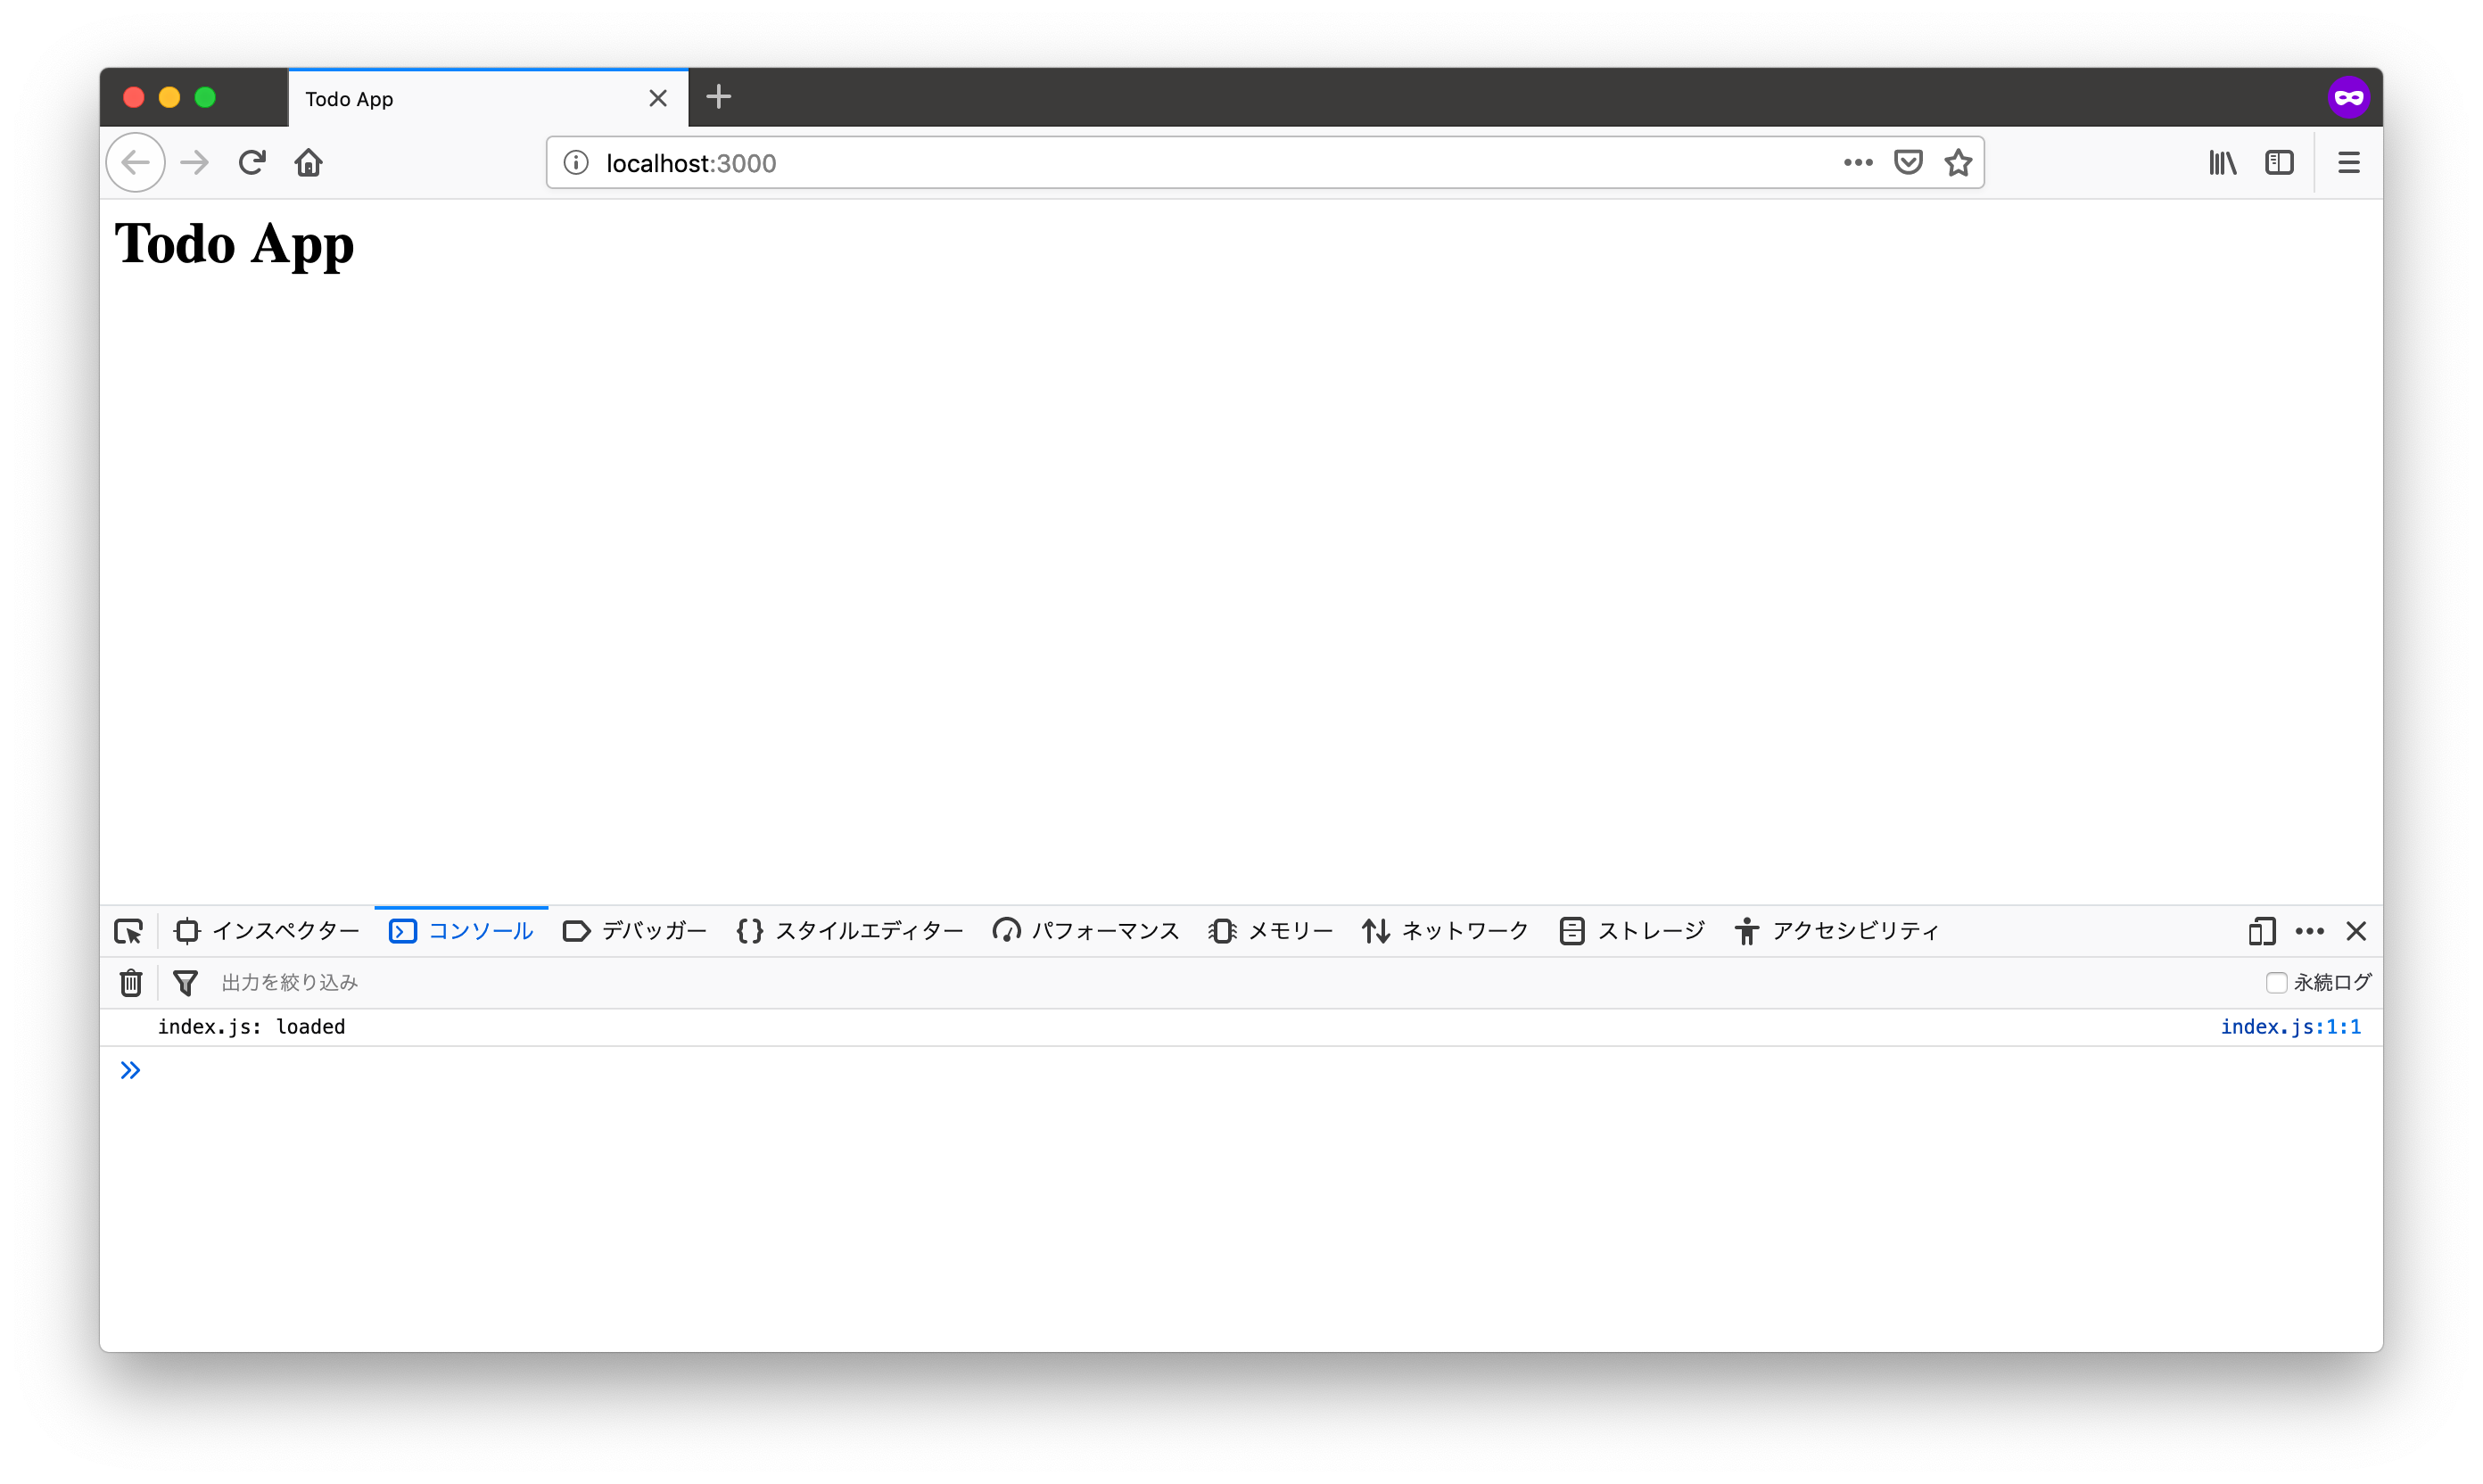
\includegraphics[width=130mm]{fig/first-entry.png}
\caption{ウェブコンソールにログが表示されている}
\end{figure}

\hypertarget{view-console-log-in-dev-tools}{%
\subsubsection{開発者ツールでのコンソールログの確認方法}\label{view-console-log-in-dev-tools}}

Console
APIで出力したログを確認するには、ウェブブラウザの開発者ツールを開く必要があります。
ほとんどのブラウザに開発者ツールが同梱されていますが、本書ではFirefoxを使って確認します。
開発者ツールの\textbf{\textgt{コンソール}}タブを開くとConsole
APIで出力したログを確認できます。

Firefoxの開発者ツールは次のいずれかの方法で開きます。

\begin{itemize}
\item
  Firefox
  メニュー(メニューバーがある場合やmacOSでは、ツールメニュー)のウェブ
  開発サブメニューで``ウェブコンソール''を選択する
\item
  キーボードショートカット\keytop{Ctrl}+\keytop{Shift}+\keytop{K}(macOSでは\keytop{Command}+\keytop{Option}+\keytop{K})を押下する
\end{itemize}

詳細はMDNの``\href{https://developer.mozilla.org/ja/docs/Tools/Web_Console/Opening_the_Web_Console}{ウェブコンソールを開く}''\footnote{\url{https://developer.mozilla.org/ja/docs/Tools/Web_Console/Opening_the_Web_Console}}を参照してください。

\hypertarget{error-not-display-console-log}{%
\subsubsection{コンソールログが表示されない}\label{error-not-display-console-log}}

HTMLは表示されるがコンソールログに\texttt{index.js: loaded}が表示されない場合は、次のような問題に該当してないかを確認してください。

\begin{description}
\item[エラー例] \texttt{index.js}\textgt{の読み込みに失敗している}\index{えらーれい@エラー例}

\texttt{script}要素の\texttt{src}属性に指定した\texttt{index.js}のパスにファイルが存在しているかを確認してください。
\texttt{<script type="module" src="index.js">}とした場合は\texttt{index.html}と\texttt{index.js}は同じディレクトリに配置する必要があります。

また、\emph{CORS policy
Invalid}のようなエラーがコンソールに表示されている場合は、\href{https://developer.mozilla.org/ja/docs/Web/Security/Same-origin_policy}{Same
Origin
Policy}により\texttt{index.js}の読み込みが失敗しています。
先ほども紹介したように、\texttt{file:}からはじまるページ上からはJavaScriptモジュールは正しく動作しません。
そのため、ローカルサーバーを起動し、ローカルサーバー(\texttt{http:}からはじまるURL)にアクセスしていることを確認してください。

\item[エラー例] \textgt{JavaScriptモジュール\index{JavaScriptもじゅーる@JavaScriptモジュール}に非対応のブラウザを利用している}

JavaScriptモジュールはまだ新しい機能であるため、バージョンが60以上のFirefoxが必要です。
バージョンが60未満のFirefoxでは、JavaScriptモジュールである\texttt{index.js}が読み込めないためコンソールログは出力されません。

今回のTodoアプリでは、ネイティブでJavaScriptモジュールに対応しているブラウザが必要です。
\href{https://caniuse.com/\#feat=es6-module}{Can I
Use}\index{Can I Use}\footnote{\url{https://caniuse.com/\#feat=es6-module}}にネイティブでJavaScriptモジュールに対応しているブラウザがまとめられています。
非対応のブラウザでもBundlerと呼ばれるツールを使うことで対応できますが、本章では省略します。
\end{description}

\hypertarget{module-entry-point}{%
\subsection{モジュールのエントリーポイントの作成}\label{module-entry-point}}\index{もじゅーる@モジュール}\index{もじゅーる@モジュール!えんとりーぽいんと@エントリーポイント}

最後にエントリーポイントとなる\texttt{index.js}から別のJavaScriptファイルをモジュールとして読み込んでみましょう。
このアプリではJavaScriptモジュールが複数登場するため\texttt{src/}というディレクトリを作り、\texttt{src/}の下にJavaScriptモジュールを書くことにします。
今回は\texttt{src/App.js}というファイルを作成し、これを\texttt{index.js}からモジュールとして読み込みます。

次のようなファイル配置となるように\texttt{src/App.js}を作成します。

\begin{lstlisting}
todoapp
├── index.html
├── index.js
└── src
      └── App.js
\end{lstlisting}

\texttt{src/App.js}ファイルを作成し、次のような内容のJavaScriptモジュールとします。
\texttt{App.js}は\texttt{App}というクラスを名前つきエクスポートしているモジュールです。
また、\texttt{App}クラスのコンストラクタにはコンソールログを出力するコードを確認用に書いておきます。

\begin{listtitle}
src/App.js
\end{listtitle}
\begin{lstlisting}
console.log("App.js: loaded");
export class App {
    constructor() {
        console.log("App initialized");
    }
}
\end{lstlisting}
\listend

次に、この\texttt{src/App.js}を\texttt{index.js}から利用するために\texttt{import}します。
\texttt{index.js}を次のように書き換え、\texttt{App.js}から\texttt{App}クラスをインポートしてインスタンス化します。

\begin{listtitle}
index.js
\end{listtitle}
\begin{lstlisting}
import { App } from "./src/App.js";
const app = new App();
\end{lstlisting}
\listend

再度ローカルサーバーのURL(\texttt{http://localhost:3000})にブラウザでアクセスし、リロードしてみましょう。
コンソールログには、次のように処理の順番どおりのログが出力されます。

\begin{lstlisting}
App.js: loaded
App initialized
\end{lstlisting}

まず\texttt{index.js}から\texttt{src/App.js}が名前つきエクスポートしている\texttt{App}クラスを名前つきインポートしています。
次に\texttt{App}クラスがインスタンス化されていることがログから確認できます。

これでHTMLとJavaScriptそれぞれのエントリーポイントの作成と動作を確認できました。

\hypertarget{error-import-app-js}{%
\subsubsection{App.jsの読み込みに失敗する}\label{error-import-app-js}}

ここまでのJavaScriptモジュールの読み込みでエラーが発生して動かない場合には、次のことを確認します。

ディレクトリ構造や\texttt{import}文で指定したファイルパスが異なると、ファイルを読み込むことができずにエラーとなってしまいます。
この場合は開発者ツールを開き、コンソールにエラーが出ていないかを確認してみてください。

\texttt{import}文\index{import@\texttt{import}}を使ったJavaScriptのモジュール読み込み時に起きる典型的なエラーと対処を次にまとめています。

\begin{description}
\item[エラー例] \textgt{SyntaxError: import declarations may only appear at top level of a module}\index{えらーれい@エラー例}

「\texttt{import}宣言はモジュールのトップレベルでしか利用できません」というエラーが出ています。
このエラーが出ているということは、\texttt{import}文を使える条件を満たしていないということです。
つまり、\texttt{import}文がトップレベルではないところに書かれている、またはモジュールではない実行コンテキストで実行されているということです。

関数の中などに\texttt{import}宣言していると、\texttt{import}宣言がトップレベルではないためエラーが発生します。
この場合は\texttt{import}文をトップレベル(プログラムの直下)に移動させてみてください。

モジュールではない実行コンテキストで実行されているというのは、裏を返せば実行コンテキストがScriptとなっているということです。
JavaScriptには実行コンテキストとしてScriptとModuleがあります。
\texttt{import}文は実行コンテキストがModuleでないと利用できません。
そのため、\texttt{script}要素の\texttt{type}属性に\texttt{module}指定を忘れていないかをチェックしてみてください。

実行コンテキストをモジュールとして実行するには\texttt{<script type="module" src="index.js">}のように\texttt{type=module}を指定する必要があります
(\texttt{index.js}から\texttt{import}文で読み込んだ\texttt{App.js}は実行コンテキストを引き継ぐため、モジュールの実行コンテキストで処理されます)。

\item[エラー例] \textgt{モジュールのソース}\texttt{``http://localhost:3000/src/App''}\textgt{の読み込みに失敗しました。}\index{えらーれい@エラー例}

\texttt{App.js}を読み込めないというエラーが出ています。
エラーメッセージをよく見ると\texttt{App}となっていて\texttt{App.js}ではありません。

\texttt{import}文では、読み込むファイルの拡張子を省略しません。
そのため、\texttt{App}のように拡張子(\texttt{.js})を省略して書いている場合はこのエラーが発生します。

\begin{lstlisting}
// エラーとなる例
import { App } from "./src/App";
\end{lstlisting}

正しくは次のように拡張子まで含めたパスを記述します。
また指定したパス(\texttt{./src/App.js})にファイルが存在するかを確認してください。

\begin{lstlisting}
// 正しい例
import { App } from "./src/App.js";
\end{lstlisting}
\end{description}

\hypertarget{conclusion}{%
\subsection{セクションのまとめ}\label{conclusion}}

このセクションでは、エントリーポイントとなるHTMLを作成し、JavaScriptモジュールのエントリーポイントとなるJavaScriptファイルを読み込むところまでを実装しました。

\hypertarget{section-checklist}{%
\subsection{このセクションのチェックリスト}\label{section-checklist}}

\begin{itemize}
\item
  \texttt{todoapp}という名前のプロジェクトディレクトリを作成した
\item
  エントリーポイントとなる\texttt{index.html}を作成した
\item
  JavaScriptのエントリーポイントとなる\texttt{index.js}を作成し\texttt{index.html}から読み込んだ
\item
  ローカルサーバーを使って\texttt{index.html}を表示した
\item
  \texttt{src/App.js}を作成し、\texttt{index.js}から\texttt{import}文で読み込めるのを確認した
\end{itemize}

ここまでのTodoアプリは次のURLで確認できます。

\begin{itemize}
\item
  \url{https://jsprimer.net/use-case/todoapp/entrypoint/module-entry/}
\end{itemize}

\hypertarget{app-structure}{%
\section{アプリの構成要素}\label{app-structure}}

HTMLとJavaScriptの\hyperlink{entrypoint_todo}{エントリーポイント}を作成しましたが、次はこのTodoアプリの構成要素を改めて見ていきましょう。

Todoアプリには、次のような機能を実装していきます。
Todoアイテムの追加、更新、削除、現在の状態の表示など複数の機能を持っています。

\begin{itemize}
\item
  Todoアイテムを追加する
\item
  Todoアイテムを更新する
\item
  Todoアイテムを削除する
\item
  Todoアイテム数(合計)の表示
\end{itemize}

また、アプリと呼ぶからには見た目もちょっとしたものにしないと雰囲気が出ません。
このセクションでは、まずウェブアプリケーションを構成するHTML、CSS、JavaScriptの役割について見ていきます。
このセクションで見た目だけで機能がないハリボテのTodoアプリを完成させ、次のセクションから実際にJavaScriptを使ってTodoアプリの機能を実装していきます。

\hypertarget{html-css-javascript}{%
\subsection{HTMLとCSSとJavaScript}\label{html-css-javascript}}\index{HTML}\index{CSS}\index{JavaScript}

Todoアプリはブラウザで動くアプリケーションとして作成しますが、ウェブアプリを作成するにはHTMLやCSS、JavaScriptを組み合わせて書いていきます。
今回はHTTP通信などはいらないクライアントサイドのみで解決するウェブアプリなので、サーバーサイドの言語は登場しません。

\begin{itemize}
\item
  \textgt{HTML}: コンテンツの構造を記述するためのマークアップ言語
\item
  \textgt{CSS}: HTMLの見た目を装飾するスタイルシート言語
\item
  \textgt{JavaScript}: インタラクションといった動作を扱うプログラミング言語
\end{itemize}

多くのウェブアプリケーションはHTMLでコンテンツの構造を定義し、CSSで見た目を装飾し、JavaScriptで動作をつけることで実装されます。
そのため、ウェブアプリはHTML、CSS、JavaScriptを組み合わせて作られています。

一方、ブラウザにはiOSやAndroidのようにOSが提供するようなUIフレームワークの標準はありません。
また、ユーザーが実装したさまざまな種類のUIフレームワークがあります。
そのため、Todoアプリという題材をとってみても、フレームワークや人によって書き方がまったく異なる場合もあります。

今回のTodoアプリは特別なUIフレームワークを使わずに、そのままのHTML、CSS、JavaScriptを組み合わせて書いていきます。

\hypertarget{todo-html}{%
\subsection{Todoアプリの構造をHTMLで定義する}\label{todo-html}}

最初に今回作成するTodoアプリのHTMLの構造を定義しています。
ここで定義したHTMLとCSSは最後までこの形のまま利用します。
次のセクションから変更していくのはJavaScriptだけということになります。

「\hyperlink{entrypoint_todo}{エントリーポイント}」のセクションで作成した\texttt{todoapp}ディレクトリの\texttt{index.html}を次の内容に変更します。

\begin{listtitle}
index.html
\end{listtitle}
\begin{lstlisting}
<html lang="ja">
  <head>
    <meta charset="UTF-8" />
    <title>Todo App</title>
    <!-- 1. CSSファイルを読み込み -->
    <link
      href="https://jsprimer.net/use-case/todoapp/final/final/index.css"
      rel="stylesheet"
    />
  </head>
  <body>
    <!-- 2. class属性をCSSのために指定 -->
    <div class="todoapp">
      <!-- 3. id属性をJavaScriptのために指定 -->
      <form id="js-form">
        <input
          id="js-form-input"
          class="new-todo"
          type="text"
          placeholder="What need to be done?"
          autocomplete="off"
        />
      </form>
      <!-- 4. TodoアプリのメインとなるTodoリスト -->
      <div id="js-todo-list" class="todo-list">
        <!-- 動的に更新されるTodoリスト -->
      </div>
      <footer class="footer">
        <!-- 5. Todoアイテム数の表示 -->
        <span id="js-todo-count">Todoアイテム数: 0</span>
      </footer>
    </div>
    <script src="./index.js" type="module"></script>
  </body>
</html>
\end{lstlisting}
\listend

HTMLの内容を変更後にブラウザでアクセスすると次のような表示になります。
まだJavaScriptでTodoアプリの機能は実装していませんが、見た目だけのTodoアプリはこれで完成です。

\begin{figure}[h]
\centering
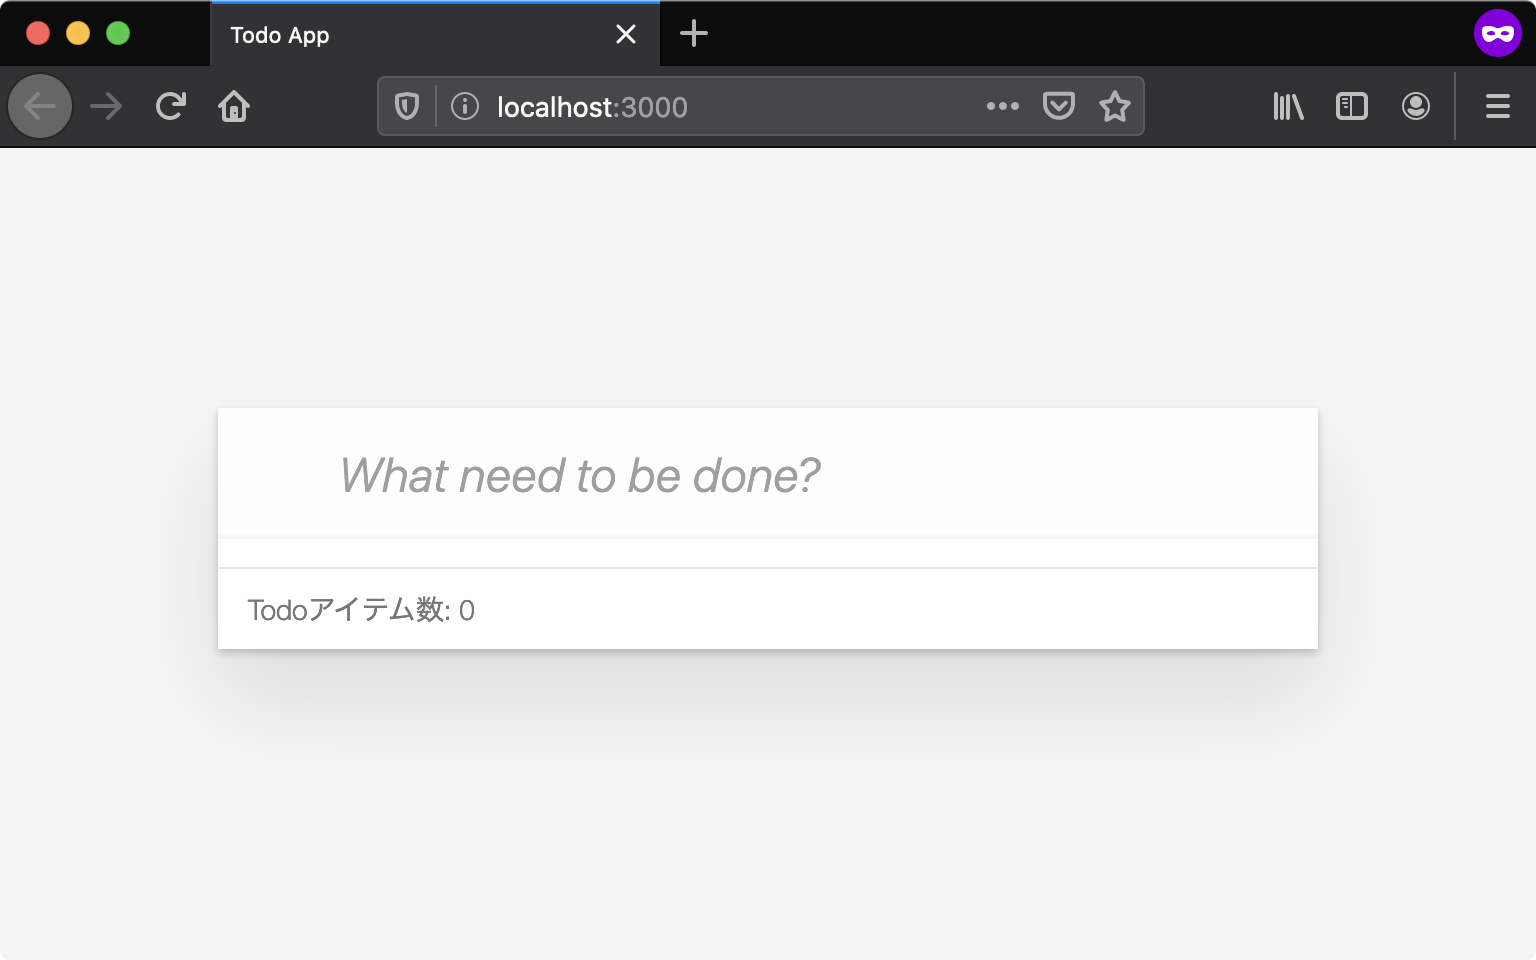
\includegraphics[width=120mm]{./fig/todo-html.png}
\caption{todoappのHTMLとCSSによる骨組み}
\end{figure}

実際に変更したHTMLを上から順番に見てみましょう。

\hypertarget{comment-css-file-load}{%
\subsubsection{1. CSSファイルを読み込み}\label{comment-css-file-load}}\index{CSS}

\texttt{head}要素の中で\texttt{link}タグを使い、外部のCSSファイルを読み込んでいます。
今回読み込んでいるCSSファイルは、Todoアプリらしい表示に必要なCSSを定義したファイルになっています。

\begin{itemize}
\item
  \url{https://jsprimer.net/use-case/todoapp/final/final/index.css}
\end{itemize}

このCSSは動作には影響がないため、今回のユースケースでは外部ファイルをそのまま取り込むだけにして解説は省略します。
CSSに定義したスタイルを正しく適用するには、\texttt{class}属性\index{classぞくせい@\texttt{class}属性}やHTML要素の構造が一致している必要があります。
表示が崩れている場合は、\texttt{class}属性が正しいか、HTMLの構造が同じになっているかを確認してください。

\hypertarget{comment-class-for-css}{%
\subsubsection{2. class属性をCSSのために指定}\label{comment-class-for-css}}\index{classぞくせい@\texttt{class}属性}

\texttt{div}\index{div@\texttt{div}}タグの\texttt{class}属性に\texttt{todoapp}という値(クラス名)を設定しています。
\texttt{class}属性は基本的にはCSSから装飾するための目印として利用されます。
また、1つのページの中で同じクラス名を複数の要素に対して設定できます。
HTMLの\texttt{class}属性はJavaScriptの\texttt{class}構文とは無関係なことには注意が必要です。

今回の\texttt{todoapp}というクラス名を持つ要素を、CSSから\texttt{.todoapp}というCSSセレクタで指定できます。
\href{https://developer.mozilla.org/ja/docs/Learn/CSS/Introduction_to_CSS/Selectors}{CSSセレクタ}\index{CSSせれくた@CSSセレクタ}とはクラス名などを使って、HTML要素を指定できる記法です。
特定の「クラス名」を持つ要素の場合は\texttt{.\hbox{}クラス名}(クラス名の前にドット)で選択できます。

次のCSSコードでは、\texttt{todoapp}というクラス名を持つ要素の\texttt{background}プロパティの値を\texttt{black}にしています。
つまり\texttt{todoapp}クラス名の要素の背景色を黒色にするという意味になります。

\begin{lstlisting}
.todoapp {
    background: black;
}
\end{lstlisting}

CSSセレクタではタグ名、\texttt{id}属性や構造などに対する指定もできます。
たとえば、特定の「id名」を持つ要素の場合は\texttt{\#id名}で選択できます。

\begin{lstlisting}
#id名 {
  /* CSSプロパティで装飾する */
}
\end{lstlisting}

\hypertarget{comment-id-for-js}{%
\subsubsection{3. id属性をJavaScriptのために指定}\label{comment-id-for-js}}\index{idぞくせい@\texttt{id}属性}

\texttt{id}属性は、その要素に対するページ内でユニークな識別子をつけるための属性です。
\texttt{id}属性はCSS、JavaScript、リンクのアンカーなど、さまざまな用途で利用されます。
また1つのページの中では同じ\texttt{id}属性名を複数の要素に対して設定できません。

今回のTodoアプリではJavaScriptから要素を選択するために\texttt{id}属性を設定しています。
先ほどのCSSセレクタはCSSから要素を指定するだけではなく、JavaScriptから要素を指定する際にも利用できます。
ブラウザのDOM APIの\texttt{document.querySelector}
APIではCSSセレクタを使って要素を選択できます。

次のコードでは、\texttt{document.querySelector("CSSセレクタ")}を利用して特定の\texttt{id}属性名の要素を取得しています。

\begin{lstlisting}
// id属性の値が"js-form"である要素を取得する
const form = document.querySelector("#js-form");
\end{lstlisting}

そのため、JavaScriptで参照する要素には\texttt{id}属性を目印としてつけています。
わかりやすくするために、JavaScriptから扱う\texttt{id}属性は慣習的に\texttt{js-}からはじまる名前にしています。

\hypertarget{comment-todo-list}{%
\subsubsection{4. TodoアプリのメインとなるTodoリスト}\label{comment-todo-list}}

\texttt{js-todo-list}という\texttt{id}属性をつけた\texttt{div}要素が、今回のTodoアプリのメインとなるTodoリストです。
この\texttt{div}要素の中身はJavaScriptで動的に更新されるため、HTMLでは目印となる\texttt{id}属性をつけています。

初期表示時はTodoリストの中身がまだ空であるため、何も表示されていません。
また\texttt{<!-\/-}と\texttt{-\/->}で囲まれた範囲はHTMLのコメントであるため、表示されません。

\hypertarget{comment-todo-count}{%
\subsubsection{5. Todoアイテム数の表示}\label{comment-todo-count}}

\texttt{js-todo-count}という\texttt{id}属性をつけた\texttt{span}\index{span@\texttt{span}}要素は、現在のTodoリストのアイテム数を表示します。
初期表示時はTodoリストが空であるため0個となりますが、Todoアイテムを追加や削除する際には合わせて更新する必要があります。

\hypertarget{conclusion}{%
\subsection{セクションのまとめ}\label{conclusion}}

このセクションではHTMLでアプリの構造を定義し、CSSでアプリのスタイルを定義しました。
次のセクションではJavaScriptモジュールを作成していき、現在は空であるTodoリストを更新していきます。

\hypertarget{section-checklist}{%
\subsection{このセクションのチェックリスト}\label{section-checklist}}

\begin{itemize}
\item
  実装するTodoアプリの構成要素を理解した
\item
  HTML、CSS、JavaScriptの役割の違いを理解した
\item
  Todoアプリの見た目をHTMLとCSSで定義した
\end{itemize}

ここまでのTodoアプリは次のURLで確認できます。

\begin{itemize}
\item
  \url{https://jsprimer.net/use-case/todoapp/app-structure/todo-html/}
\end{itemize}

\hypertarget{form-event}{%
\section{Todoアイテムの追加を実装する}\label{form-event}}

ここからはJavaScriptでTodoアプリの機能を作成していきます。

このセクションでは、前のセクションでHTMLに目印をつけたTodoリスト(\texttt{\#js-todo-list})に対してTodoアイテムを追加する処理を実装します。

\hypertarget{add-todo-item}{%
\subsection{Todoアイテムの追加}\label{add-todo-item}}

まず、Todoアプリではどのような操作をしたら、Todoアイテムを追加できるかを見ていきます。

Todoアプリでは、ユーザーが次のような操作を行った場合に、Todoアイテムを追加します。

\begin{enumerate}
\def\labelenumi{\arabic{enumi}.}
\item
  入力欄にTodoアイテムのタイトルを入力する
\item
  入力欄で\keytop{Enter}キーを押して送信する
\item
  TodoリストにTodoアイテムが追加される
\end{enumerate}

これをJavaScriptで実現するには次のことが必要です。

\begin{itemize}
\item
  Todoアイテムのタイトルを取得するために、input要素(入力欄)から内容を取得する
\item
  \keytop{Enter}キーで送信されたことを知るために、form要素の\texttt{submit}イベント(送信)を監視する
\item
  入力内容をタイトルにしたTodoアイテムを作成し、Todoリスト(\texttt{\#js-todo-list})にTodoアイテム要素を追加する
\end{itemize}

まずは、form要素から送信されたイベントを受け取り、入力内容をコンソールログに表示してみることからはじめてみましょう。

\hypertarget{input-to-console}{%
\subsection{入力内容をコンソールに表示する}\label{input-to-console}}

form\index{form@\texttt{form}}要素で\keytop{Enter}キーを押して送信すると\texttt{submit}\index{submit@\texttt{submit}}イベントが発生します。
この\texttt{submit}イベントはHTML要素の\texttt{addEventListener}\index{addEventListener@\texttt{addEventListener}}メソッドを利用することで受け取れます。

次のコードでは、指定したform要素から\texttt{submit}イベントが発生したときに呼び出されるコールバック関数を登録しています。

\begin{lstlisting}
// id="js-form"の要素を取得
const formElement = document.querySelector("#js-form");
// form要素から発生したsubmitイベントを受け取る
formElement.addEventListener("submit", (event) => {
    // イベントが発生したときに呼ばれるコールバック関数(イベントリスナー)
});
\end{lstlisting}

このようなイベントが発生した際に呼ばれるコールバック関数のことを\textbf{\textgt{イベントリスナー}}\index{いべんとりすなー@イベントリスナー}(イベントをリッスンするものという意味)と呼びます。
またイベントリスナーはイベントハンドラー\index{いべんとはんどらー@イベントハンドラー}とも呼ばれることがありますが、この書籍ではこの2つの言葉は同じ意味として扱います。

フォームが送信されたときに入力内容をコンソールに表示するには、
\texttt{addEventListener}コールバック関数内で入力内容をConsole
APIで出力すればよいことになります。

入力内容はinput要素の\texttt{value}プロパティから取得できます。

\begin{lstlisting}
const inputElement = document.querySelector("#js-form-input");
console.log(inputElement.value); // => "input要素の入力内容"
\end{lstlisting}

これらを組み合わせて\texttt{App.js}に「入力内容をコンソールに表示」する機能を実装してみましょう。
\texttt{App}クラスに\texttt{mount}というメソッドを定義して、その中に処理を書いていきます。

次のコードでは、フォーム(\texttt{\#js-form})を\keytop{Enter}で送信すると、input\index{input@\texttt{input}}要素(\texttt{\#js-form-input})の内容をコンソールへ表示する処理を実装しています。

\begin{listtitle}
src/App.js
\end{listtitle}
\begin{lstlisting}
export class App {
    mount() {
        const formElement = document.querySelector("#js-form");
        const inputElement = document.querySelector("#js-form-input");
        formElement.addEventListener("submit", (event) => {
            // submitイベントの本来の動作を止める
            event.preventDefault();
            console.log(`入力欄の値: ${inputElement.value}`);
        });
    }
}
\end{lstlisting}
\listend

このままでは、\texttt{App\#mount}は呼び出されないため何も行われません。
そのため、\texttt{index.js}も変更して、\texttt{App}クラスの\texttt{mount}メソッドを呼び出すようにします。

\begin{listtitle}
index.js
\end{listtitle}
\begin{lstlisting}
import { App } from "./src/App.js";
const app = new App();
app.mount();
\end{lstlisting}
\listend

これらの変更後にブラウザでページをリロードすると、\texttt{App\#mount}メソッドが実行されるようになります。
\texttt{submit}イベントがリッスンされているので、入力欄に何か入力して\keytop{Enter}で送信してみるとその内容がコンソールに表示されます。

\begin{figure}[h]
\centering
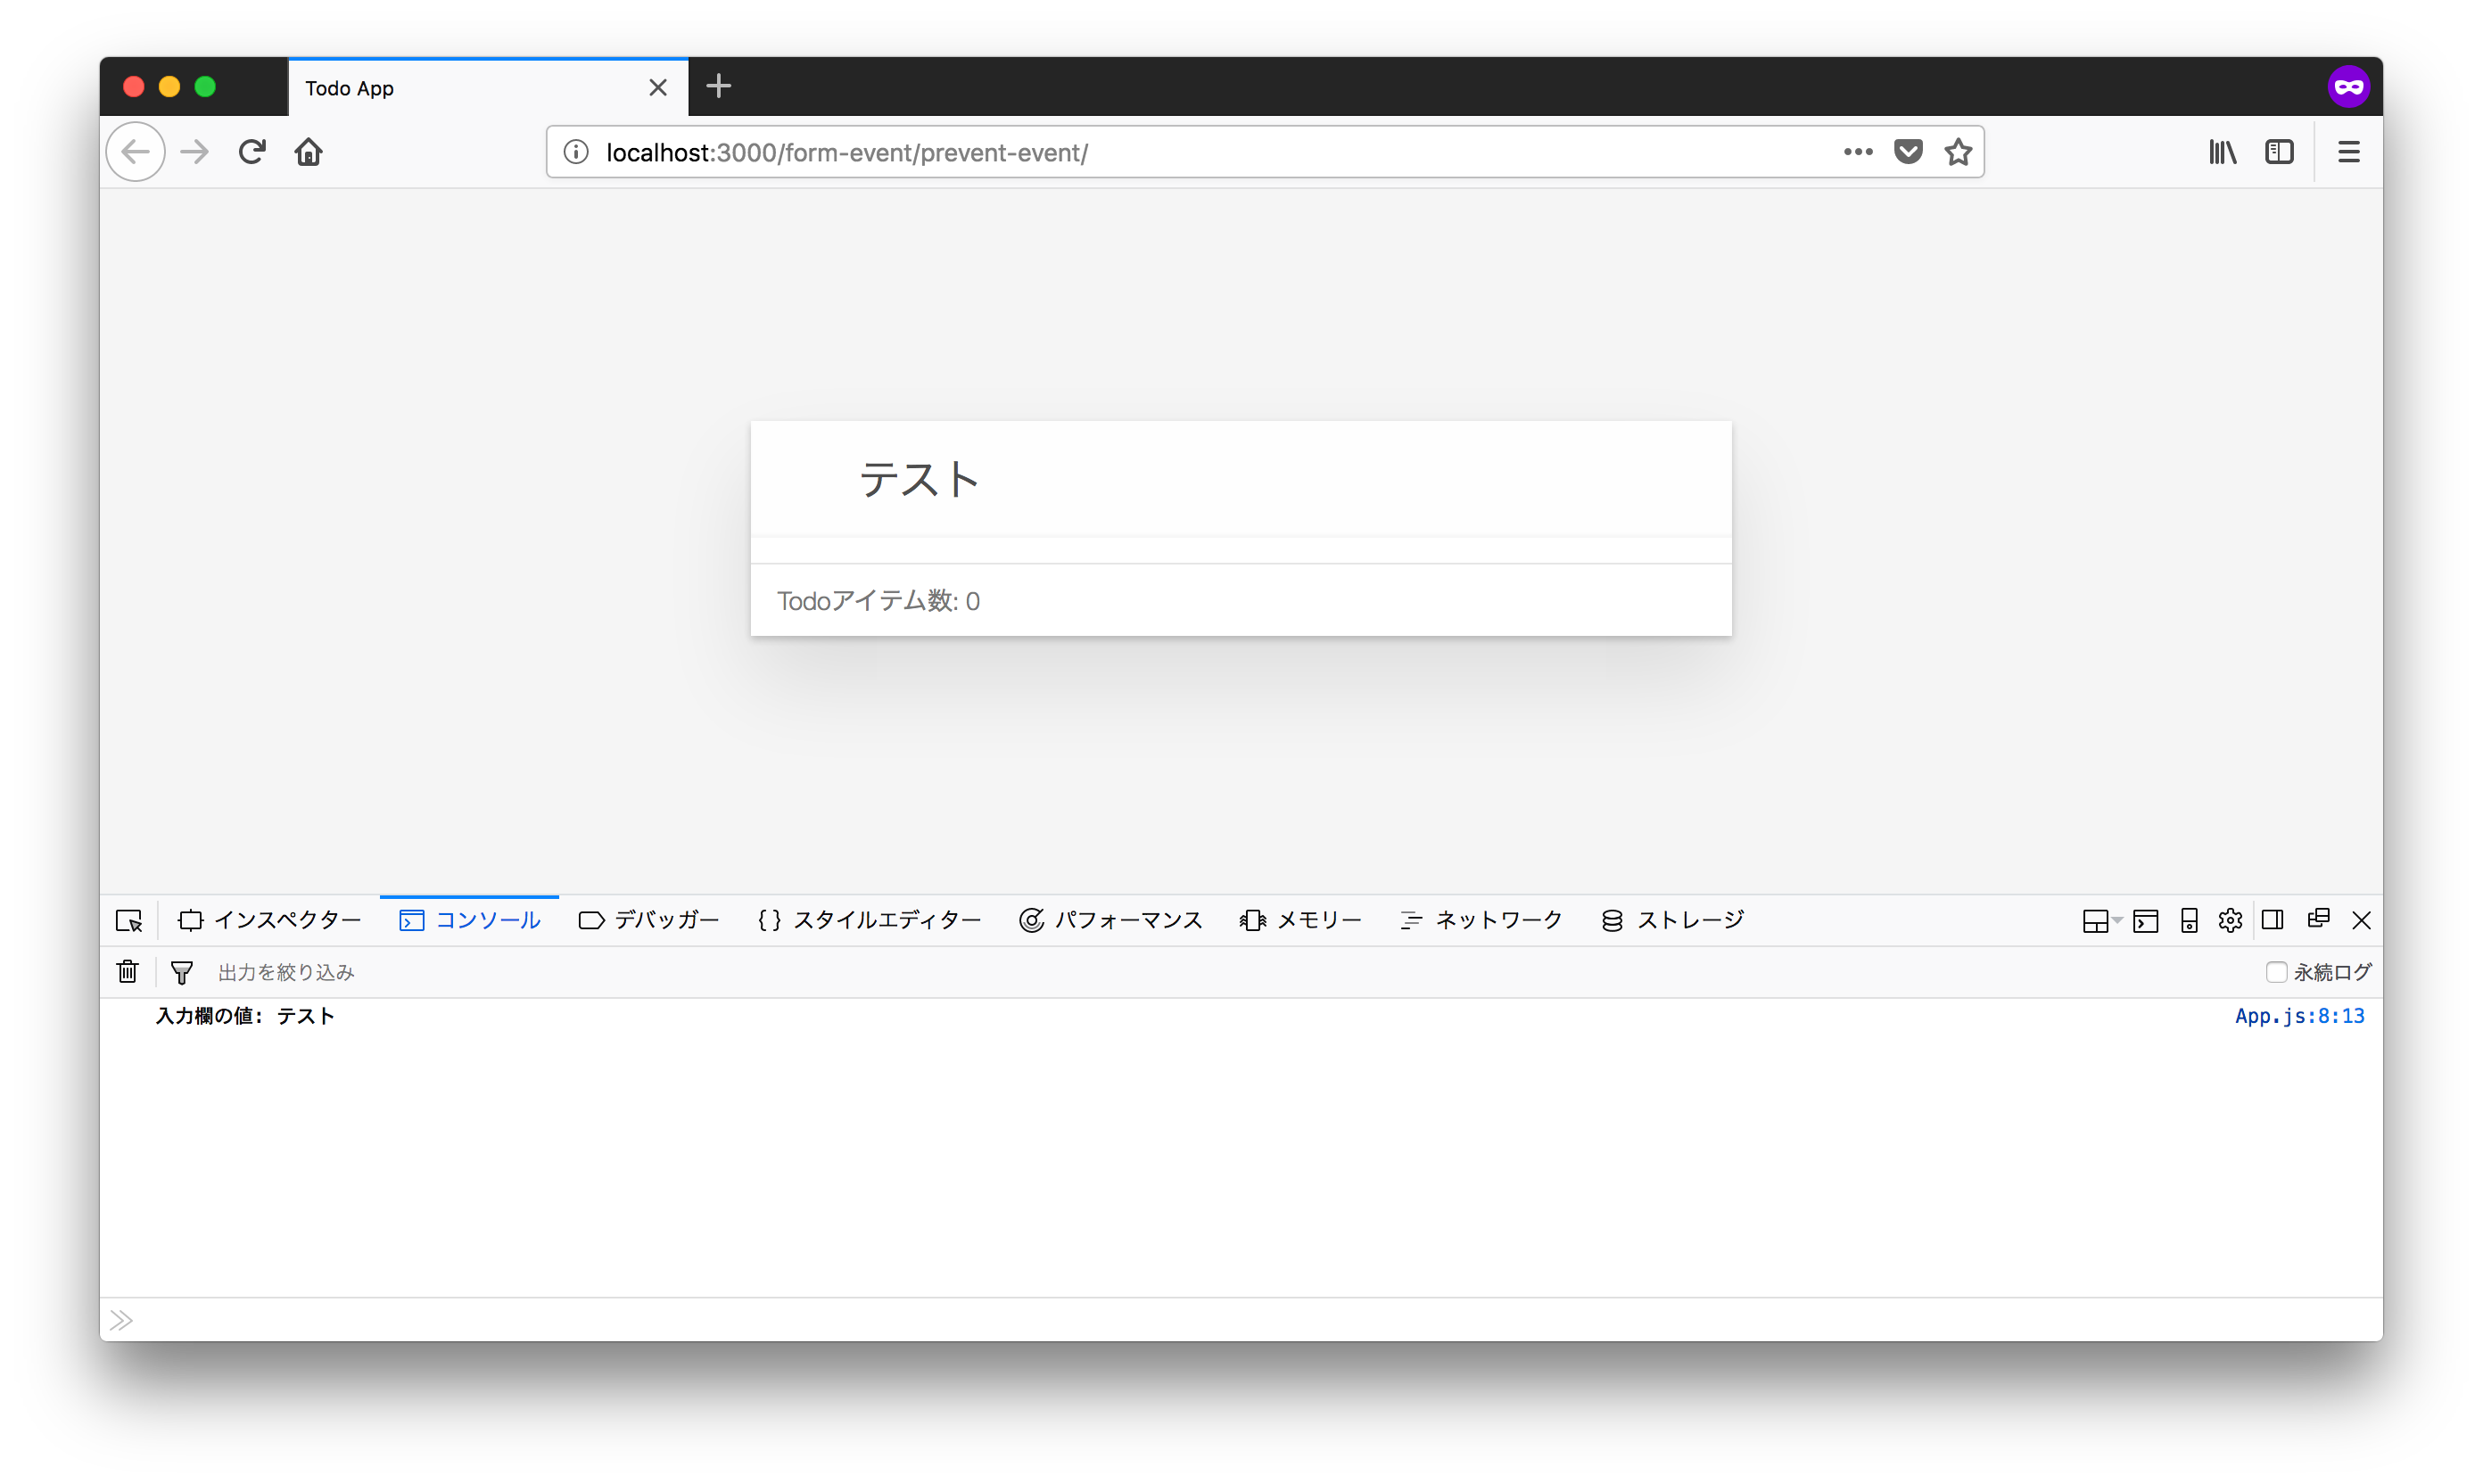
\includegraphics[width=130mm]{./fig/form-event.png}
\caption{入力内容がコンソールに表示される}
\end{figure}

先ほどの\texttt{App\#mount}メソッドでは、\texttt{submit}イベントのイベントリスナー内で\texttt{event.preventDefault}メソッドを呼び出しています。
\texttt{event.preventDefault}\index{event.preventDefault@\texttt{event.preventDefault}}メソッドは、\texttt{submit}イベントの発生元であるフォームが持つデフォルトの動作をキャンセルするメソッドです。

フォームが持つデフォルトの動作とは、フォームの内容を指定したURLへ送信するという動作です。
ここでは\texttt{form}要素に送信先が指定されていないため、現在のURLに対してフォームの内容を送信します。
しかしこの動作は邪魔になるため、\texttt{event.preventDefault}メソッドを呼び出すことで、このデフォルトの動作をキャンセルしています。

\begin{listtitle}
src/App.jsより抜粋
\end{listtitle}
\begin{lstlisting}
formElement.addEventListener("submit", (event) => {
    // submitイベントの本来の動作を止める
    event.preventDefault();
    console.log(`入力欄の値: ${inputElement.value}`);
});
\end{lstlisting}
\listend

現在のURLに対してフォームの送信が行われると、結果的にページがリロードされてしまいます。
そのため、\texttt{event.preventDefault()}を呼び出し、デフォルトの動作をキャンセルしていました。
\texttt{event.preventDefault()}をコメントアウトすると、ページがリロードされてしまうことが確認できます。

\begin{listtitle}
src/App.jsから一部をコメントアウトした例
\end{listtitle}
\begin{lstlisting}
formElement.addEventListener("submit", (event) => {
    // preventDefaultしないとページがリロードされてしまう
    // event.preventDefault();
    console.log(`入力欄の値: ${inputElement.value}`);
});
\end{lstlisting}
\listend

ここまでで\texttt{todoapp}ディレクトリに、次のような変更を加えました。

\begin{lstlisting}
todoapp
├── index.html
├── index.js (App#mountの呼び出し)
└── src
      └── App.js (App#mountの実装)
\end{lstlisting}

ここまでのTodoアプリは次のURLで確認できます。

\begin{itemize}
\item
  \url{https://jsprimer.net/use-case/todoapp/form-event/prevent-event/}
\end{itemize}

\hypertarget{input-to-todolist}{%
\subsection{入力内容をTodoリストに表示する}\label{input-to-todolist}}

フォーム送信時に入力内容を取得する方法がわかったので、次はその入力内容をTodoリスト(\texttt{\#js-todo-list})に表示します。

HTMLではリストのアイテムを記述する際には\texttt{<li>}\index{<li>@\texttt{<li>}}タグを使います。
また後ほどTodoリストに表示するTodoアイテムの要素には、完了状態を表すチェックボックスや削除ボタンなども含めたいです。
これらの要素を含むものを手続き的にDOM
APIで作成すると見通しが悪くなるため、HTML文字列からHTML要素を生成するユーティリティモジュールを作成しましょう。

次の\texttt{html-util.js}というファイルを\texttt{src/view/html-util.js}というパスに作成します。

この\texttt{html-util.js}は「\hyperlink{usecase-ajax}{Ajax通信}」の「\hyperlink{html-to-dom}{HTML文字列をDOMに追加する}」でも利用した\texttt{escapeSpecialChars}をベースにしています。
ajaxappでの\texttt{escapeHTML}タグ関数では出力は\textbf{\textgt{HTML文字列}}でしたが、今回作成する\texttt{element}タグ関数の出力は\textbf{\textgt{HTML要素}}(Element)です。

Todoリスト(\texttt{\#js-todo-list})というすでに存在する要素に対して要素を\textbf{\textgt{追加}}するには、HTML文字列ではなくHTML要素が必要になります。
また、HTML文字列に対しては\texttt{addEventListener}でイベントをリッスンできません。
そのため、チェックボックスの状態が変わったことや削除ボタンが押されたことを知る必要があるTodoアプリではHTML要素が必要になります。

\begin{listtitle}
src/view/html-util.js
\end{listtitle}
\begin{lstlisting}
export function escapeSpecialChars(str) {
    return str
        .replace(/&/g, "&amp;")
        .replace(/</g, "&lt;")
        .replace(/>/g, "&gt;")
        .replace(/"/g, "&quot;")
        .replace(/'/g, "&#039;");
}

/**
 * HTML文字列からHTML要素を作成して返す
 * @param {string} html 
 */
export function htmlToElement(html) {
    const template = document.createElement("template");
    template.innerHTML = html;
    return template.content.firstElementChild;
}

/**
 * HTML文字列からDOM Nodeを作成して返すタグ関数
 * @return {Element}
 */
export function element(strings, ...values) {
    const htmlString = strings.reduce((result, str, i) => {
        const value = values[i - 1];
        if (typeof value === "string") {
            return result + escapeSpecialChars(value) + str;
        } else {
            return result + String(value) + str;
        }
    });
    return htmlToElement(htmlString);
}

/**
 * コンテナ要素の中身をbodyElementで上書きする
 * @param {Element} bodyElement コンテナ要素の中身となる要素
 * @param {Element} containerElement コンテナ要素
 */
export function render(bodyElement, containerElement) {
    // containerElementの中身を空にする
    containerElement.innerHTML = "";
    // containerElementの直下にbodyElementを追加する
    containerElement.appendChild(bodyElement);
}
\end{lstlisting}
\listend

\texttt{element}タグ関数では、同じファイルに定義した\texttt{htmlToElement}関数を使ってHTML文字列からHTML要素を作成しています。
\texttt{htmlToElement}関数の中で利用している\href{https://developer.mozilla.org/ja/docs/Web/HTML/Element/template}{\texttt{template}要素}\index{template@\texttt{template}}はHTML5で追加された、HTML文字列の断片からHTML要素を作成できる要素です。

この\texttt{element}タグ関数を使うことで、次のようにHTML文字列からHTML要素を作成できます。
作成した要素は、\texttt{appendChild}\index{appendChild@\texttt{appendChild}}メソッドなどで既存の要素に子要素として追加できます。

\begin{listtitle}
elementタグ関数のサンプルコード
\end{listtitle}
\begin{lstlisting}
// HTML文字列からHTML要素を作成
const newElement = element`<ul>
    <li>新しい要素</li>
</ul>`;
// 作成した要素をdocument.bodyの子要素として追加(appendChild)する
document.body.appendChild(newElement);
\end{lstlisting}
\listend

ブラウザが提供する\texttt{appendChild}メソッドは子要素を追加するだけなので、すでに別の要素がある場合は末尾に追加されます。

このセクションではまだ利用しませんが、\texttt{html-util.js}には\texttt{render}という関数を定義しています。
\texttt{render}関数は指定したコンテナ要素(親となる要素)の子要素を上書きする関数となります。
動作的には一度子要素をすべて消したあとに\texttt{appendChild}で子要素として追加しています。

\begin{listtitle}
render関数のサンプルコード
\end{listtitle}
\begin{lstlisting}
// ul要素の空タグを作成
const newElement = element`<ul />`;
// newElementをdocument.bodyの子要素として追加する
// すでにdocument.body以下に要素がある場合は上書きされる
render(newElement, document.body);
\end{lstlisting}
\listend

最後に、この\texttt{element}タグ関数を使って、フォームから送信された入力内容をTodoリストに要素として追加してみます。

\texttt{App.js}から先ほど作成した\texttt{html-util.js}の\texttt{element}タグ関数を\texttt{import}します。
次に\texttt{submit}イベントのリスナー関数で、Todoアイテムを表現する要素を作成し、Todoリスト(\texttt{\#js-todo-list})の子要素として追加(\texttt{appendChild})します。
最後にTodoアイテム数(\texttt{\#js-todo-count})のテキスト(\texttt{textContent})を更新します。

\begin{listtitle}
src/App.js
\end{listtitle}
\begin{lstlisting}
import { element } from "./view/html-util.js";

export class App {
    mount() {
        const formElement = document.querySelector("#js-form");
        const inputElement = document.querySelector("#js-form-input");
        const containerElement = document.querySelector("#js-todo-list");
        const todoItemCountElement = document.querySelector("#js-todo-count");
        // Todoアイテム数
        let todoItemCount = 0;
        formElement.addEventListener("submit", (event) => {
            // 本来のsubmitイベントの動作を止める
            event.preventDefault();
            // 追加するTodoアイテムの要素(li要素)を作成する
            const todoItemElement = element`<li>${inputElement.value}</li>`;
            // Todoアイテムをcontainerに追加する
            containerElement.appendChild(todoItemElement);
            // Todoアイテム数を+1し、表示されてるテキストを更新する
            todoItemCount += 1;
            todoItemCountElement.textContent = `Todoアイテム数: ${todoItemCount}`;
            // 入力欄を空文字列にしてリセットする
            inputElement.value = "";
        });
    }
}
\end{lstlisting}
\listend

これらの変更後にブラウザでページをリロードし、フォームに入力してから\keytop{Enter}を押すとTodoリストに\textbf{\textgt{Todoアイテムが追加}}されます。
また、入力内容を送信するたびに\texttt{todoItemCount}が加算され、\textbf{\textgt{Todoアイテム数}}の表示も更新されます。

\begin{figure}[h]
\centering
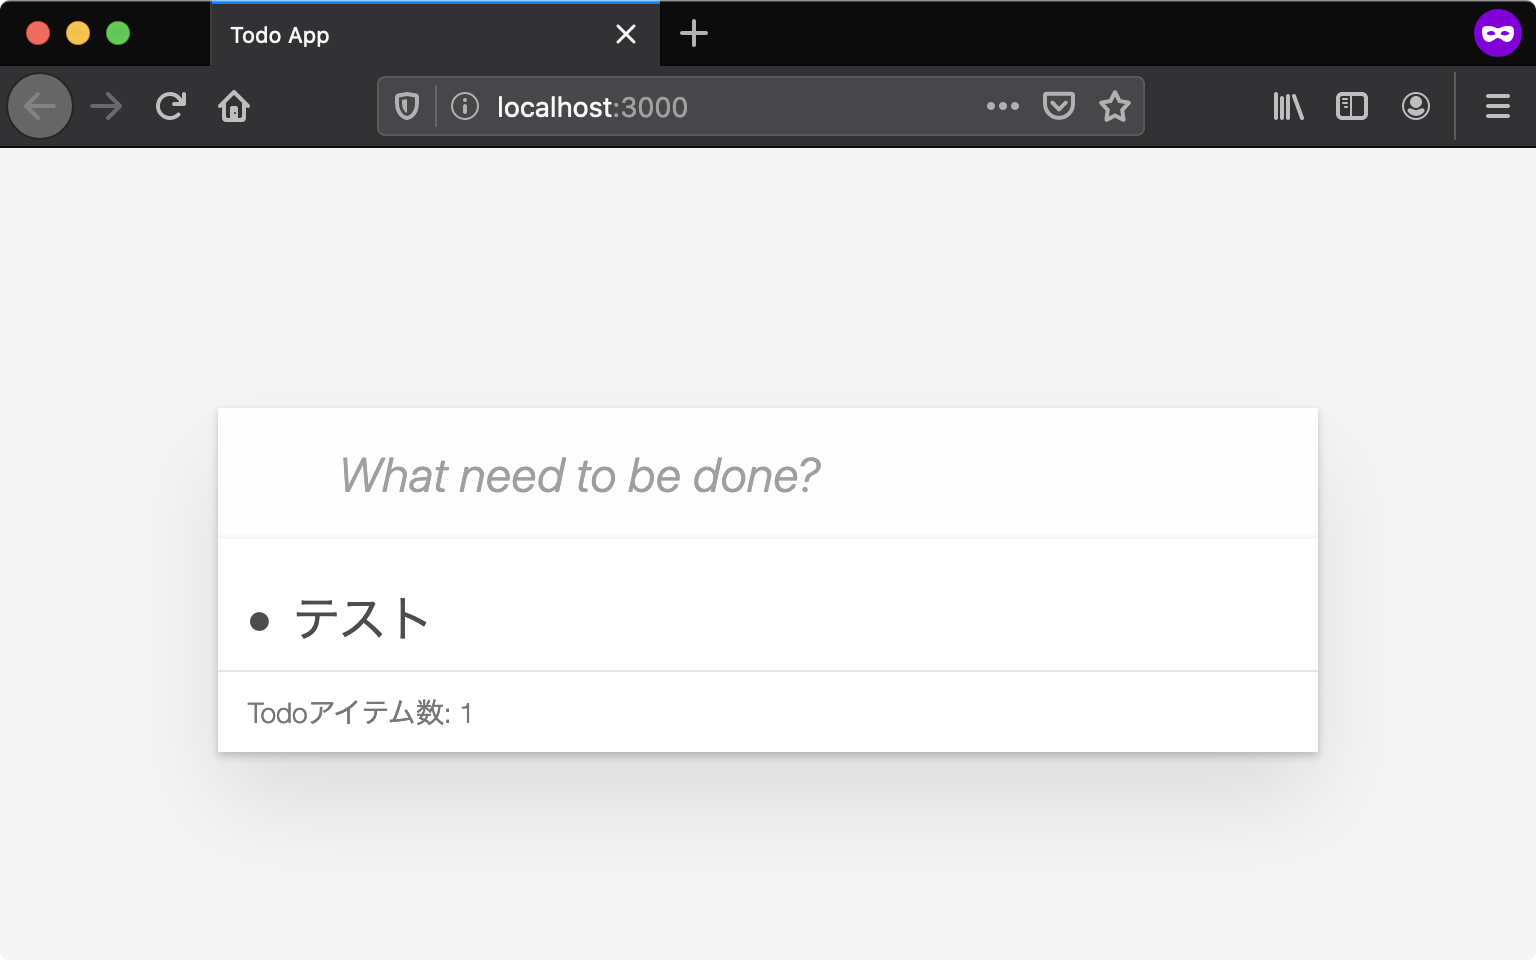
\includegraphics[width=120mm]{./fig/add-todo-item.png}
\caption{Todoリストへアイテムを追加}
\end{figure}

\newpage
このセクションでの変更点は次のとおりです。

\begin{lstlisting}
todoapp
├── index.html
├── index.js
└── src
      ├── App.js(Todoアイテムの表示の実装)
      └── view
            └── html-util.js(新規追加)
\end{lstlisting}

ここまでのTodoアプリは次のURLで確認できます。

\begin{itemize}
\item
  \url{https://jsprimer.net/use-case/todoapp/form-event/add-todo-item/}
\end{itemize}

\hypertarget{conclusion}{%
\subsection{セクションのまとめ}\label{conclusion}}

このセクションではform要素の\texttt{submit}イベントをリッスンし、入力内容を元にTodoアイテムを作成し、これをTodoリストに追加する機能を実装しました。
今回のTodoアイテムの追加のように、多くのウェブアプリは何らかのイベントをリッスンして表示を更新します。
このような、イベントが発生したことを元に処理を進める方法を\textbf{\textgt{イベント駆動}}\index{いべんとくどう@イベント駆動}(イベントドリブン\index{いべんとどりぶん@イベントドリブン})と呼びます。

今回のTodoアイテムの追加では、\texttt{submit}イベントを入力にして、Todoリスト要素を\textbf{\textgt{直接HTML要素として追加}}するという方法を取っていました。
このように直接DOMを更新するという方法はコードが短くなりますが、DOMのみにしか状態が残らないため柔軟性がなくなるという問題があります。
次のセクションでは、実際に起きる問題やそれを解決するための仕組みを見ていきます。

\hypertarget{section-checklist}{%
\subsection{このセクションのチェックリスト}\label{section-checklist}}

\begin{itemize}
\item
  フォームの送信を\texttt{submit}イベントで受け取り、入力内容を確認した
\item
  HTML文字列からHTML要素を作成する\texttt{html-util.js}を実装した
\item
  フォームからTodoアイテムを追加した
\item
  Todoアイテムの追加に合わせてTodoアイテム数を更新した
\end{itemize}

このセクションで、TodoアプリにTodoアイテムを追加する機能が実装できました。

\begin{itemize}
\item
  Todoアイテムを追加できる
\end{itemize}

Todoアプリに実装する残りの機能は次のとおりです。

\begin{itemize}
\item
  Todoアイテムの完了状態を更新できる
\item
  Todoアイテムを削除できる
\end{itemize}

\hypertarget{event-model}{%
\section{イベントとモデル}\label{event-model}}\index{いべんと@イベント}\index{もでる@モデル}

Todoアイテムを追加する機能を実装しましたが、イベントを受け取って直接DOMを更新する方法には柔軟性がないという問題があります。
また「Todoアイテムの更新」という機能を実装するには、追加したTodoアイテム要素を識別する方法が必要です。
具体的には、Todoアイテムごとに\texttt{id}属性などのユニークな識別子がないため、特定のアイテムを指定して更新や削除をする機能が実装できません。

このセクションでは、まずどのような点で柔軟性の問題が起きやすいのかを見ていきます。
そして、柔軟性や識別子の問題を解決するために\textbf{\textgt{モデル}}という概念を導入し、「Todoアイテムの追加」の機能をリファクタリングしていきます。

\hypertarget{direct-dom-modification-issue}{%
\subsection{直接DOMを更新する問題}\label{direct-dom-modification-issue}}

「\hyperlink{form-event}{Todoアイテムの追加を実装する}」では、操作した結果発生したイベントという入力に対して、DOM(表示)を直接更新していました。
そのため、TodoリストにTodoアイテムが何個あるか、どのようなアイテムがあるかという状態がDOM上にしか存在しないことになります。

この場合にTodoアイテムの状態を更新するには、HTML要素にTodoアイテムの情報(タイトルや識別子となるidなど)をすべて埋め込む必要があります。
しかし、HTML要素は文字列しか扱えないため、Todoアイテムのデータを文字列にしないといけないという制限が発生します。

また、1つの操作に対して複数の箇所の表示が更新されることもあります。
今回のTodoアプリでもTodoリスト(\texttt{\#js-todo-list})とTodoアイテム数(\texttt{\#js-todo-count})の2箇所を更新する必要があります。

次の表に\textbf{\textgt{操作}}に対して更新する\textbf{\textgt{表示}}をまとめてみます。

\begin{small}
\begin{longtable}[l]{p{30mm}|p{30mm}|p{80mm}}
\hline\rowcolor[gray]{0.85}\rule[0mm]{0mm}{4mm}{\textgt 機能} & {\textgt 操作} & {\textgt 表示}\tabularnewline
\hline
\endhead
Todoアイテムの追加 & フォームを入力して送信 & Todoリスト(\texttt{\#js-todo-list})にTodoアイテム要素を作成して子要素として追加。合わせてTodoアイテム数(\texttt{\#js-todo-count})を更新\tabularnewline
Todoアイテムの更新 & チェックボックスをクリック & Todoリスト(\texttt{\#js-todo-list})にある指定したTodoアイテム要素のチェック状態を更新\tabularnewline
Todoアイテムの削除 & 削除ボタンをクリック & Todoリスト(\texttt{\#js-todo-list})にある指定したTodoアイテム要素を削除。合わせてTodoアイテム数(\texttt{\#js-todo-count})を更新\tabularnewline
\hline
\end{longtable}
\end{small}

1つの操作に対する表示の更新箇所が増えるほど、操作に対する処理(リスナーの処理)が複雑化していくことが予想できます。

ここでは、次の2つの問題が見つかりました。

\begin{itemize}
\item
  Todoリストの状態がDOM上にしか存在しないため、状態をすべてDOM上に文字列で埋め込まないといけない
\item
  操作に対して更新する表示箇所が増えてくると、表示の処理が複雑化する
\end{itemize}

\hypertarget{introduce-model}{%
\subsection{モデルを導入する}\label{introduce-model}}

この問題を避けるために、Todoアイテムという情報をJavaScriptクラスとしてモデル化します。
ここでのモデルとはTodoアイテムやTodoリストなどの\textbf{\textgt{モノの状態\index{じょうたい@状態}や操作方法}}を定義したオブジェクトという意味です。
クラスでは操作方法はメソッドとして実装し、状態はインスタンスのプロパティで管理できるため、今回はクラスでモデルを表現します。

たとえば、Todoリストを表現するモデルとして\texttt{TodoListModel}クラスを考えます。
TodoリストにはTodoアイテムを追加できるので、\texttt{TodoListModel\#addItem}というメソッドがあると良さそうです。
また、Todoリストからアイテムの一覧を取得できる必要もあるので、\texttt{TodoListModel\#getAllItems}というメソッドも必要そうです。
このようにTodoリストをクラスで表現する際に、オブジェクトがどのような処理や状態を持つかを考えて実装します。

このようにモデルを考えた後、先ほどの操作と表示の間にモデルを入れることを考えてみます。
「フォームを入力して送信」という\textbf{\textgt{操作}}をした場合には、\texttt{TodoListModel}(Todoリスト)に対して\texttt{TodoItemModel}(Todoアイテム)を追加します。
そして、\texttt{TodoListModel}からTodoアイテムの一覧を取得し、それを元にDOMを組み立て、\textbf{\textgt{表示}}を更新します。

先ほどの表にモデルを入れてみます。
\textbf{\textgt{操作}}に対する\textbf{\textgt{モデルの処理}}はさまざまですが、\textbf{\textgt{操作}}に対する\textbf{\textgt{表示}}の処理はどの場合も同じになります。
これは表示箇所が増えた場合でも\textbf{\textgt{表示}}の処理の複雑さが一定に保てることを意味しています。

\begin{small}
\begin{longtable}[l]{p{30mm}|p{30mm}|p{50mm}|p{30mm}}
\hline\rowcolor[gray]{0.85}\rule[0mm]{0mm}{4mm}{\textgt 機能} & {\textgt 操作} & {\textgt モデルの処理} & {\textgt 表示}\tabularnewline
\hline
\endhead
Todoアイテムの追加 & フォームを入力して送信 & \texttt{TodoListModel}へ新しい\texttt{TodoItem Model}を追加 & \texttt{TodoListModel}を元に表示を更新\tabularnewline
Todoアイテムの更新 & チェックボックスをクリック & \texttt{TodoListModel}の指定した\texttt{TodoIt emModel}の状態を更新 & \texttt{TodoListModel}を元に表示を更新\tabularnewline
Todoアイテムの削除 & 削除ボタンをクリック & \texttt{TodoListModel}から指定の\texttt{TodoIt emModel}を削除 & \texttt{TodoListModel}を元に表示を更新\tabularnewline
\hline
\end{longtable}
\end{small}

この表を元に改めて先ほどの問題点を見ていきましょう。

\begin{itemize}
\item Todoリストの状態がDOM上にしか存在しないため、状態をすべてDOM上に文字列で埋め込まないといけない
\end{itemize}

モデルであるクラスのインスタンスを参照すれば、Todoアイテムの情報が手に入ります。
またモデルはただのJavaScriptクラスであるため、文字列ではない情報も保持できます。
そのため、DOMにすべての情報を埋め込む必要はありません。

\begin{itemize}
\item 操作に対して更新する表示箇所が増えてくると、表示の処理が複雑化する
\end{itemize}

モデルの状態を元にしてHTML要素を作成し、表示を更新します。
モデルの状態が変化していなければ、表示は変わらなくても問題ありません。

そのため操作したタイミングではなく、モデルの状態が変化したタイミングで表示を更新すればよいはずです。
具体的には「フォームを入力して送信」されたから表示を更新するのではなく、
「\texttt{TodoListModel}というモデルの状態が変化」したから表示を更新すればいいはずです。

そのためには、\texttt{TodoListModel}というモデルの状態が変化したことを表示側から知る必要があります。
ここで再び出てくるのがイベントです。

\hypertarget{model-and-event}{%
\subsection{モデルの変化を伝えるイベント}\label{model-and-event}}\index{いべんと@イベント}

フォームを送信したらform要素から\texttt{submit}イベントが発生します。
これと同じように\texttt{TodoListModel}の状態が変化したら自分自身へ\texttt{change}\index{change@\texttt{change}}イベントを発生(ディスパッチ\index{でぃすぱっち@ディスパッチ})させます。
表示側はそのイベントをリッスン\index{りっすん@リッスン}してイベントが発生したら表示を更新すればよいはずです。

\texttt{TodoListModel}の状態の変化とは、「\texttt{TodoListModel}に新しい\texttt{TodoItemModel}が追加される」などが該当します。
先ほどの表の「モデルの処理」は何かしら状態が変化しているので、表示を更新する必要があるわけです。

DOM
APIのイベントの仕組みをモデルでも利用できれば、モデルが更新されたら表示を更新する仕組みを作れそうです。
ブラウザのDOM APIでは、DOM
Events\index{DOM Events}と呼ばれるイベントの仕組みが利用できます。
Node.jsでは、\texttt{events}\index{events@\texttt{events}}と呼ばれる組み込みのモジュールで同様のイベントの仕組みが利用できます。

実行環境が提供するイベントの仕組みを利用すると簡単ですが、ここではイベントの仕組みを理解するために、イベントのディスパッチとリッスンする機能を持つクラスを作ってみましょう。

とても難しく聞こえますが、今まで学んだクラスやコールバック関数などを使えば実現できます。

\hypertarget{event-emitter}{%
\subsection{EventEmitter}\label{event-emitter}}\index{EventEmitter}

イベントの仕組みとは「イベントをディスパッチする側」と「イベントをリッスンする側」の2つの面から成り立ちます。
場合によっては自分自身へイベントをディスパッチし、自分自身でイベントをリッスンすることもあります。

このイベントの仕組みを言い換えると「イベントをディスパッチした(イベントを発生させた)ときにイベントをリッスンしているコールバック関数(イベントリスナー)を呼び出す」となります。

モデルが更新されたら表示を更新するには「\texttt{TodoListModel}が更新されたときに指定したコールバック関数を呼び出すクラス」を作れば目的は達成できます。
しかし、「\texttt{TodoListModel}が更新されたとき」というのはとても具体的な処理であるため、モデルを増やすたびに同じ処理をそれぞれのモデルへ実装するのは大変です。

そのため、先ほどのイベントの仕組みを持った概念として\texttt{EventEmitter}というクラスを作成します。
そして\texttt{TodoListModel}には作成した\texttt{EventEmitter}を継承することでイベントの仕組みを導入していきます。

\begin{itemize}
\item
  \textgt{親クラス}(\texttt{EventEmitter}): 
  イベントをディスパッチしたとき、登録されているコールバック関数(イベントリスナー)を呼び出すクラス
\item
  \textgt{子クラス}(\texttt{TodoListModel}): 
  値を更新したとき、登録されているコールバック関数を呼び出すクラス
\end{itemize}

まずは、親クラスとなる\texttt{EventEmitter}を作成していきます。

\texttt{EventEmitter}はイベントの仕組みで書いたディスパッチ側とリッスン側の機能を持ったクラスとなります。

\begin{itemize}
\item
  \textgt{ディスパッチ側}:
  \texttt{emit}\index{emit@\texttt{emit}}メソッドは、指定された\texttt{イベント名}に登録済みのすべてのコールバック関数を呼び出す
\item
  \textgt{リッスン側}:
  \texttt{addEventListener}\index{addEventListener@\texttt{addEventListener}}メソッドは、指定した\texttt{イベント名}に任意のコールバック関数を登録できる
\end{itemize}

これによって、\texttt{emit}メソッドを呼び出すと指定したイベントに関係する登録済みのコールバック関数を呼び出せます。
このようなパターンはObserverパターン\index{Observerぱたーん@Observerパターン}とも呼ばれ、ブラウザやNode.jsなど多くの実行環境に類似するAPIが存在します。

次のように\texttt{src/EventEmitter.js}へ\texttt{EventEmitter}クラスを定義します。

\begin{listtitle}
src/EventEmitter.js
\end{listtitle}
\begin{lstlisting}
export class EventEmitter {
    constructor() {
        // 登録する [イベント名, Set(リスナー関数)] を管理するMap
        this._listeners = new Map();
    }

    /**
     * 指定したイベントが実行されたときに呼び出されるリスナー関数を登録する
     * @param {string} type イベント名
     * @param {Function} listener イベントリスナー
     */
    addEventListener(type, listener) {
        // 指定したイベントに対応するSetを作成し、リスナー関数を登録する
        if (!this._listeners.has(type)) {
            this._listeners.set(type, new Set());
        }
        const listenerSet = this._listeners.get(type);
        listenerSet.add(listener);
    }

    /**
     * 指定したイベントをディスパッチする
     * @param {string} type イベント名
     */
    emit(type) {
        // 指定したイベントに対応するSetを取り出し、すべてのリスナー関数を呼び出す
        const listenerSet = this._listeners.get(type);
        if (!listenerSet) {
            return;
        }
        listenerSet.forEach(listener => {
            listener.call(this);
        });
    }

    /**
     * 指定したイベントのイベントリスナーを解除する
     * @param {string} type イベント名
     * @param {Function} listener イベントリスナー
     */
    removeEventListener(type, listener) {
        // 指定したイベントに対応するSetを取り出し、該当するリスナー関数を削除する
        const listenerSet = this._listeners.get(type);
        if (!listenerSet) {
            return;
        }
        listenerSet.forEach(ownListener => {
            if (ownListener === listener) {
                listenerSet.delete(listener);
            }
        });
    }
}
\end{lstlisting}
\listend

この\texttt{EventEmitter}では、次のようにイベントのリッスンとイベントのディスパッチの機能が利用できます。
リッスン側は\texttt{addEventListener}メソッドでイベントの種類(\texttt{type})に対するイベントリスナー(\texttt{listener})を登録します。
ディスパッチ側は\texttt{emit}メソッドでイベントをディスパッチし、イベントリスナーを呼び出します。

次のコードでは、\texttt{addEventListener}メソッドで\texttt{test-event}イベントに対して2つのイベントリスナーを登録しています。
そのため、\texttt{emit}メソッドで\texttt{test-event}イベントをディスパッチすると、登録済みのイベントリスナーが呼び出されています。

\begin{listtitle}
EventEmitterの実行サンプル
\end{listtitle}
\begin{lstlisting}
import { EventEmitter } from "./EventEmitter.js";
const event = new EventEmitter();
// イベントリスナー(コールバック関数)を登録
event.addEventListener("test-event", () => console.log("One!"));
event.addEventListener("test-event", () => console.log("Two!"));
// イベントをディスパッチする
event.emit("test-event");
// コールバック関数がそれぞれ呼びだされ、コンソールには次のように出力される
// "One!"
// "Two!"
\end{lstlisting}
\listend

\hypertarget{event-emitter-todolist-model}{%
\subsection{EventEmitterを継承したTodoListモデル}\label{event-emitter-todolist-model}}

次は作成した\texttt{EventEmitter}クラスを継承した\texttt{TodoListModel}クラスを作成しています。
\texttt{src/model/}ディレクトリを新たに作成し、このディレクトリに各モデルクラスを実装したファイルを作成します。

作成するモデルは、Todoリストを表現する\texttt{TodoListModel}と各Todoアイテムを表現する\texttt{TodoItemModel}です。
\texttt{TodoListModel}が複数の\texttt{TodoItemModel}を保持することでTodoリストを表現します。

\begin{itemize}
\item
  \texttt{TodoListModel}: Todoリストを表現するモデル
\item
  \texttt{TodoItemModel}: Todoアイテムを表現するモデル
\end{itemize}

まずは\texttt{TodoItemModel}を\texttt{src/model/TodoItemModel.js}というファイル名で作成します。

\texttt{TodoItemModel}クラスは各Todoアイテムに必要な情報を定義します。
各Todoアイテムにはタイトル(\texttt{title})、アイテムの完了状態(\texttt{completed})、アイテムごとにユニークな識別子(\texttt{id})を持たせます。
ただのデータの集合であるため、クラスではなくオブジェクトでも問題はありませんが、今回はクラスとして作成します。

次のように\texttt{src/model/TodoItemModel.js}へ\texttt{TodoItemModel}クラスを定義します。

\begin{listtitle}
src/model/TodoItemModel.js
\end{listtitle}
\begin{lstlisting}
// ユニークなIDを管理する変数
let todoIdx = 0;

export class TodoItemModel {
    /**
     * @param {string} title Todoアイテムのタイトル
     * @param {boolean} completed Todoアイテムが完了済みならばtrue、
     * そうでない場合はfalse
     */
    constructor({ title, completed }) {
        // idは自動的に連番となりそれぞれのインスタンスごとに異なるものとする
        this.id = todoIdx++;
        this.title = title;
        this.completed = completed;
    }
}
\end{lstlisting}
\listend

次のコードでは\texttt{TodoItemModel}クラスはインスタンス化でき、それぞれの\texttt{id}が自動的に異なる値となっていることが確認できます。
この\texttt{id}は後ほど特定のTodoアイテムを指定して更新する処理のときに、アイテムを区別する識別子として利用します。

\begin{listtitle}
TodoItemModel.jsを利用するサンプルコード
\end{listtitle}
\begin{lstlisting}
import { TodoItemModel } from "./TodoItemModel.js";
const item = new TodoItemModel({
    title: "未完了のTodoアイテム",
    completed: false
});
const completedItem = new TodoItemModel({
    title: "完了済みのTodoアイテム",
    completed: true
});
// それぞれのidは異なる
console.log(item.id !== completedItem.id); // => true
\end{lstlisting}
\listend

次に\texttt{TodoListModel}を\texttt{src/model/TodoListModel.js}というファイル名で作成します。

\texttt{TodoListModel}クラスは、先ほど作成した\texttt{EventEmitter}クラスを継承します。
\texttt{TodoListModel}クラスは\texttt{TodoItemModel}の配列を保持し、新しいTodoアイテムを追加する際はその配列に追加します。
このとき\texttt{TodoListModel}の状態が変更したことを通知するために自分自身へ\texttt{change}イベントをディスパッチします。

\begin{listtitle}
src/model/TodoListModel.js
\end{listtitle}
\begin{lstlisting}
import { EventEmitter } from "../EventEmitter.js";

export class TodoListModel extends EventEmitter {
    /**
     * @param {TodoItemModel[]} [items] 初期アイテム一覧(デフォルトは空の配列)
     */
    constructor(items = []) {
        super();
        this.items = items;
    }

    /**
     * TodoItemの合計個数を返す
     * @returns {number}
     */
    getTotalCount() {
        return this.items.length;
    }

    /**
     * 表示できるTodoItemの配列を返す
     * @returns {TodoItemModel[]}
     */
    getTodoItems() {
        return this.items;
    }

    /**
     * TodoListの状態が更新されたときに呼び出されるリスナー関数を登録する
     * @param {Function} listener
     */
    onChange(listener) {
        this.addEventListener("change", listener);
    }

    /**
     * 状態が変更されたときに呼ぶ。登録済みのリスナー関数を呼び出す
     */
    emitChange() {
        this.emit("change");
    }

    /**
     * TodoItemを追加する
     * @param {TodoItemModel} todoItem
     */
    addTodo(todoItem) {
        this.items.push(todoItem);
        this.emitChange();
    }
}
\end{lstlisting}
\listend

次のコードは\texttt{TodoListModel}クラスのインスタンスに対して、新しい\texttt{TodoItemModel}を追加するサンプルコードです。
\texttt{TodoListModel\#addTodo}メソッドで新しいTodoアイテムを追加したときに、\texttt{TodoListModel\#onChange}で登録したイベントリスナーが呼び出されます。

\begin{listtitle}
TodoListModel.jsを利用するサンプルコード
\end{listtitle}
\begin{lstlisting}
import { TodoItemModel } from "./TodoItemModel.js";
import { TodoListModel } from "./TodoListModel.js";
// 新しいTodoリストを作成する
const todoListModel = new TodoListModel();
// 現在のTodoアイテム数は0
console.log(todoListModel.getTotalCount()); // => 0
// Todoリストが変更されたら呼ばれるイベントリスナーを登録する
todoListModel.onChange(() => {
    console.log("TodoListの状態が変わりました");
});
// 新しいTodoアイテムを追加する
// => onChangeで登録したイベントリスナーが呼び出される
todoListModel.addTodo(new TodoItemModel({
    title: "新しいTodoアイテム",
    completed: false
}));
// Todoリストにアイテムが増える
console.log(todoListModel.getTotalCount()); // => 1
\end{lstlisting}
\listend

これでTodoリストに必要なそれぞれのモデルクラスが作成できました。
次はこれらのモデルを使って、表示の更新をしてみましょう。

\hypertarget{model-update-view}{%
\subsection{モデルを使って表示を更新する}\label{model-update-view}}

先ほど作成した\texttt{TodoListModel}と\texttt{TodoItemModel}クラスを使って、「Todoアイテムの追加」を書き直してみます。

前回のコードでは、フォームを送信すると直接DOMへ要素を追加していました。
今回のコードでは、フォームを送信すると\texttt{TodoListModel}へ\texttt{TodoItemModel}を追加します。
\texttt{TodoListModel}に新しいTodoアイテムが増えると、\texttt{onChange}に登録したイベントリスナーが呼び出されるため、
そのリスナー関数内でDOM(表示)を更新します。

まずは書き換え後の\texttt{App.js}を見ていきます。

\begin{listtitle}
src/App.js
\end{listtitle}
\begin{lstlisting}
import { TodoListModel } from "./model/TodoListModel.js";
import { TodoItemModel } from "./model/TodoItemModel.js";
import { element, render } from "./view/html-util.js";

export class App {
    constructor() {
        // 1. TodoListの初期化
        this.todoListModel = new TodoListModel();
    }
    mount() {
        const formElement = document.querySelector("#js-form");
        const inputElement = document.querySelector("#js-form-input");
        const containerElement = document.querySelector("#js-todo-list");
        const todoItemCountElement = document.querySelector("#js-todo-count");
        // 2. TodoListModelの状態が更新されたら表示を更新する
        this.todoListModel.onChange(() => {
            // TodoリストをまとめるList要素
            const todoListElement = element`<ul />`;
            // それぞれのTodoItem要素をtodoListElement以下へ追加する
            const todoItems = this.todoListModel.getTodoItems();
            todoItems.forEach(item => {
                const todoItemElement = element`<li>${item.title}</li>`;
                todoListElement.appendChild(todoItemElement);
            });
            // containerElementの中身をtodoListElementで上書きする
            render(todoListElement, containerElement);
            // アイテム数の表示を更新
            todoItemCountElement.textContent = `Todoアイテム数: 
                                      ${this.todoListModel.getTotalCount()}`;
        });
        // 3. フォームを送信したら、新しいTodoItemModelを追加する
        formElement.addEventListener("submit", (event) => {
            event.preventDefault();
            // 新しいTodoItemをTodoListへ追加する
            this.todoListModel.addTodo(new TodoItemModel({
                title: inputElement.value,
                completed: false
            }));
            inputElement.value = "";
        });
    }
}
\end{lstlisting}
\listend

変更後の\texttt{App.js}では大きく分けて3つの部分が変更されているので、順番に見ていきます。

\hypertarget{app-todolist-initialize}{%
\subsubsection{1. TodoListの初期化}\label{app-todolist-initialize}}

作成した\texttt{TodoListModel}と\texttt{TodoItemModel}をインポートしています。

\begin{lstlisting}
import { TodoListModel } from "./model/TodoListModel.js";
import { TodoItemModel } from "./model/TodoItemModel.js";
\end{lstlisting}

そして、\texttt{App}クラスのコンストラクタ内で\texttt{TodoListModel}を初期化しています。
\texttt{App}のコンストラクタで\texttt{TodoListModel}を初期化しているのは、
このTodoアプリでは開始時にTodoリストの中身が空の状態で開始されるのに合わせるためです。

\begin{listtitle}
src/App.jsより抜粋
\end{listtitle}
\begin{lstlisting}
// ...省略...
export class App {
    constructor() {
        // 1. TodoListの初期化
        this.todoListModel = new TodoListModel();
    }
    // ...省略...
}
\end{lstlisting}
\listend

\hypertarget{app-todolist-onchange}{%
\subsubsection{2. TodoListModelの状態が更新されたら表示を更新する}\label{app-todolist-onchange}}

\texttt{mount}メソッド内で\texttt{TodoListModel}が更新されたら表示を更新するという処理を実装します。
\texttt{TodoListModel\#onChange}で登録したリスナー関数は、\texttt{TodoListModel}の状態が更新されたら呼び出されます。

このリスナー関数内では\texttt{TodoListModel\#getTodoItems}でTodoアイテムを取得しています。
そして、アイテム一覧から次のようなリスト要素(\texttt{todoListElement})を作成しています。

\begin{lstlisting}[language=HTML]
<!-- todoListElementの実質的な中身 -->
<ul>
    <li>Todoアイテム 1のタイトル</li>
    <li>Todoアイテム 2のタイトル</li>
</ul>
\end{lstlisting}

この作成した\texttt{todoListElement}要素を、前回作成した\texttt{html-util.js}の\texttt{render}関数を使って\texttt{containerElement}の中身に上書きしています。
また、アイテム数は\texttt{TodoListModel\#getTotalCount}メソッドで取得できるため、アイテム数を管理していた\texttt{todoItemCount}という変数は削除できます。

\begin{listtitle}
src/App.jsより抜粋
\end{listtitle}
\begin{lstlisting}
// render関数をimportに追加する
import { element, render } from "./view/html-util.js";
export class App {
    // ...省略...
    mount() {
        // ...省略...
        this.todoListModel.onChange(() => {
            // ...省略...
            // containerElementの中身をtodoListElementで上書きする
            render(todoListElement, containerElement);
            // アイテム数の表示を更新
            todoItemCountElement.textContent = `Todoアイテム数: 
                                      ${this.todoListModel.getTotalCount()}`;
        });
        // ...省略...
    }
}
\end{lstlisting}
\listend

\hypertarget{app-add-new-todoitem}{%
\subsubsection{3. フォームを送信したら、新しいTodoItemを追加する}\label{app-add-new-todoitem}}

前回のコードでは、フォームを送信(\texttt{submit})すると直接DOMへ要素を追加していました。
今回のコードでは、\texttt{TodoListModel}の状態が更新されたら表示を更新する仕組みがすでにできています。

そのため、\texttt{submit}イベントのリスナー関数内では\texttt{TodoListModel}に対して新しい\texttt{TodoItemModel}を追加するだけで表示が更新されます。
直接DOMへ\texttt{appendChild}していた部分を\texttt{TodoListModel\#addTodo}メソッドを使ってモデルを更新する処理へ置き換えるだけです。

\hypertarget{conclusion}{%
\subsection{セクションのまとめ}\label{conclusion}}

今回のセクションでは、前セクションの「\hyperlink{form-event}{Todoアイテムの追加を実装する}」をモデルとイベントの仕組みを使うようにリファクタリングしました。
コード量は増えましたが、次に実装する「Todoアイテムの更新」や「Todoアイテムの削除」も同様の仕組みで実装できます。
前回のセクションのように操作に対してDOMを直接更新した場合、追加は簡単ですが既存の要素を指定する必要がある更新や削除は難しくなります。

次のセクションでは、残りの機能である「Todoアイテムの更新」や「Todoアイテムの削除」を実装していきます。

\hypertarget{section-checklist}{%
\subsection{このセクションのチェックリスト}\label{section-checklist}}

\begin{itemize}
\item
  直接DOMを更新する問題について理解した
\item
  \texttt{EventEmitter}クラスでイベントの仕組みを実装した
\item
  TodoリストとTodoアイテムをモデルとして実装した
\item
  \texttt{TodoListModel}を\texttt{EventEmitter}クラスを継承して実装した
\item
  Todoアイテムの追加の機能をモデルを使ってリファクタリングした
\end{itemize}

ここまでのTodoアプリは次のURLで確認できます。

\begin{itemize}
\item
  \url{https://jsprimer.net/use-case/todoapp/event-model/event-emitter/}
\end{itemize}

\hypertarget{todo-item-update-and-delete}{%
\section{Todoアイテムの更新と削除を実装する}\label{todo-item-update-and-delete}}

このセクションでは、Todoアプリの残りの機能である「Todoアイテムの更新」と「Todoアイテムの削除」を実装していきます。

「Todoアイテムの更新」とは、チェックボックスをクリックして未完了だったらチェックをつけて完了済みに、逆に完了済みのアイテムを未完了へとトグルする機能のことです。完了状態をTodoアイテムごとに持ち、それぞれのTodoの進捗を管理できる機能です。

一方の「Todoアイテムの削除」はボタンをクリックしたらTodoアイテムを削除する機能です。
不要となったTodoを削除して完了済みのTodoを取り除くなどに利用できる機能です。

まずは「Todoアイテムの更新」から実装します。その後「Todoアイテムの削除」を実装していきます。

\hypertarget{todo-item-update}{%
\subsection{Todoアイテムの更新}\label{todo-item-update}}

現時点ではTodoアイテムが完了済みかどうかの状態が表示されていません。
そのため、まずはTodoアイテムが完了済みかを表示する必要があります。
HTMLの\href{https://developer.mozilla.org/ja/docs/Web/HTML/Element/Input/checkbox}{\texttt{<input type="checkbox">}}要素を使ってチェックボックスを表示し、Todoアイテムごとの完了状態を表現します。

\texttt{<input type="checkbox">}は\texttt{checked}属性\index{checkedぞくせい@\texttt{checked}属性}がない場合はチェックが外れた状態のチェックボックスとなります。
一方\texttt{<input type="checkbox" checked>}のように\texttt{checked}属性がある場合はチェックがついたチェックボックスとなります。

\begin{figure}[h]
\centering
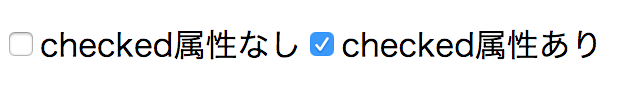
\includegraphics[width=100mm]{./fig/input-checkbox.png}
\caption{input要素のchecked属性の違い}
\end{figure}

\texttt{src/App.js}の\texttt{TodoListModel\#onChange}メソッドで登録したリスナー関数内を書き換え、チェックボックスを表示しています。

Todoアイテム要素である\texttt{<li>}\index{<li>@\texttt{<li>}}要素中に次のように\texttt{<input>}要素を追加してチェックボックスを表示に追加します。
チェックボックスである\texttt{<input>}\index{<input>@\texttt{<input>}}要素にはスタイルのために\texttt{class}属性\index{classぞくせい@\texttt{class}属性}を\texttt{checkbox}\index{checkbox@\texttt{checkbox}}とします。
合わせて完了済みの場合は\texttt{<s>}\index{<s>@\texttt{<s>}}要素を使って打ち消し線を表示しています。

\begin{listtitle}
src/App.jsから抜粋
\end{listtitle}
\begin{lstlisting}
        this.todoListModel.onChange(() => {
            const todoListElement = element`<ul />`;
            const todoItems = this.todoListModel.getTodoItems();
            todoItems.forEach(item => {
                // 完了済みならchecked属性をつけ、未完了ならchecked属性を外す
                // input要素にはcheckboxクラスをつける
                const todoItemElement = item.completed
                    ? element`<li><input type="checkbox" 
                             class="checkbox" checked><s>${item.title}
                             </s></input></li>`
                    : element`<li><input type="checkbox" 
                             class="checkbox">${item.title}
                             </input></li>`;
                todoListElement.appendChild(todoItemElement);
            });
            render(todoListElement, containerElement);
            todoItemCountElement.textContent = `Todoアイテム数: 
                                     ${this.todoListModel.getTotalCount()}`;
        });
\end{lstlisting}
\listend

\texttt{<input type="checkbox">}要素はクリックするとチェックの表示がトグルします。
しかし、モデルである\texttt{TodoItemModel}の\texttt{completed}プロパティの状態は自動では切り替わりません。
これにより表示とモデルの状態が異なってしまうという問題が発生します。

この問題は次のような操作をしてみると確認できます。

\begin{enumerate}
\def\labelenumi{\arabic{enumi}.}
\item
  Todoアイテムを追加する
\item
  Todoアイテムのチェックボックスにチェックをつける
\item
  別の新しいTodoアイテムを追加する
\item
  すべてのチェックボックスのチェックがリセットされてしまう
\end{enumerate}

この問題を避けるためにも、\texttt{<input type="checkbox">}要素がチェックされたらモデルの状態を更新する必要があります。

\texttt{<input type="checkbox">}要素はチェックされたときに\texttt{change}イベントをディスパッチします。
この\texttt{change}イベントをリッスンして、TodoItemモデルの状態を更新すればモデルと表示の状態を同期できます。

\texttt{input}要素からディスパッチされる\texttt{change}イベントをリッスンする処理は次のように書けます。

まずは\texttt{todoItemElement}要素の下にある\texttt{input}要素を\texttt{querySelector}\index{querySelector@\texttt{querySelector}}メソッドで探索します。
以前は\texttt{document.querySelector}で\texttt{document}以下からCSSセレクタにマッチする要素を探索していました。
\texttt{todoItemElement.querySelector}メソッドを使うことで、\texttt{todoItemElement}下にある要素だけを対象に探索できます。

そして、見つけた\texttt{input}要素に対して\texttt{addEventListener}メソッドで\texttt{change}イベントが発生したときに呼ばれるコールバック関数を登録できます。

\begin{lstlisting}
const todoItemElement = element`<li><input type="checkbox" class="checkbox">
                               ${item.title}</input></li>`;
// クラス名checkboxを持つ要素を取得
const inputCheckboxElement = todoItemElement.querySelector(".checkbox");
// <input type="checkbox">のチェックが変更されたときに呼ばれるイベントリスナーを
// 登録
inputCheckboxElement.addEventListener("change", () => {
    // チェックボックスの表示が変わったタイミングで呼び出される処理
    // TODO: ここでモデルを更新する処理を呼ぶ
});
\end{lstlisting}

ここまでをまとめると、Todoアイテムの更新は次の2つのステップで実装できます。

\begin{enumerate}
\def\labelenumi{\arabic{enumi}.}
\item
  \texttt{TodoListModel}に指定したTodoアイテムの更新処理を追加する
\item
  チェックボックスの\texttt{change}イベントが発生したら、モデルの状態を更新する
\end{enumerate}

ここから実際にTodoアイテムの更新を\texttt{todoapp}プロジェクトに実装していきます。

\hypertarget{TodoListModel-updateTodo}{%
\subsubsection{\texorpdfstring{\texttt{TodoListModel}に指定したTodoアイテムの更新処理を追加する}{TodoListModelに指定したTodoアイテムの更新処理を追加する}}\label{TodoListModel-updateTodo}}

まずは、\texttt{TodoListModel}に指定したTodoアイテムを更新する\texttt{updateTodo}メソッドを追加します。
\texttt{TodoListModel\#updateTodo}メソッドは、指定したidと一致するTodoアイテムの完了状態(\texttt{completed}プロパティ)を更新します。

\begin{listtitle}
src/model/TodoListModel.jsの変更点を抜粋
\end{listtitle}
\begin{lstlisting}
    // ===============================
    // TodoListModel.jsの既存の実装は省略
    // ===============================
    /**
     * 指定したidのTodoItemのcompletedを更新する
     * @param {{ id:number, completed: boolean }}
     */
    updateTodo({ id, completed }) {
        // idが一致するTodoItemを見つけ、あるなら完了状態の値を更新する
        const todoItem = this.items.find(todo => todo.id === id);
        if (!todoItem) {
            return;
        }
        todoItem.completed = completed;
        this.emitChange();
    }
}
\end{lstlisting}
\listend

\hypertarget{onChange-update-model}{%
\subsubsection{\texorpdfstring{チェックボックスの\texttt{change}イベントが発生したら、Todoアイテムの完了状態を更新する}{チェックボックスのchangeイベントが発生したら、Todoアイテムの完了状態を更新する}}\label{onChange-update-model}}

次に\texttt{input}要素の\texttt{change}イベントのリスナー関数で、Todoアイテムの完了状態を更新します。

\texttt{src/App.js}の\texttt{TodoListModel\#onChange}メソッドで登録したリスナー関数内を次のように書き換えます。

\texttt{App.js}で\texttt{todoItemElement}の子要素として\texttt{checkbox}というクラス名をつけた\texttt{input}要素を追加します。
この\texttt{input}要素の\texttt{change}イベントが発生したら、\texttt{TodoListModel\#updateTodo}メソッドを呼び出すようにします。
チェックがトグルするたびに呼び出されるので、\texttt{completed}には現在の状態を反転(トグル)した値を渡します。

\begin{listtitle}
src/App.jsから変更点を抜粋
\end{listtitle}
\begin{lstlisting}
        this.todoListModel.onChange(() => {
            const todoListElement = element`<ul />`;
            const todoItems = this.todoListModel.getTodoItems();
            todoItems.forEach(item => {
                // 完了済みならchecked属性をつけ、未完了ならchecked属性を外す
                const todoItemElement = item.completed
                    ? element`<li><input type="checkbox" 
                             class="checkbox" checked><s>${item.title}
                             </s></input></li>`
                    : element`<li><input type="checkbox" class="checkbox">
                             ${item.title}</input></li>`;
                // チェックボックスがトグルしたときのイベントにリスナー関数を登録
                const inputCheckboxElement = 
                                  todoItemElement.querySelector(".checkbox");
                inputCheckboxElement.addEventListener("change", () => {
                    // 指定したTodoアイテムの完了状態を反転させる
                    this.todoListModel.updateTodo({
                        id: item.id,
                        completed: !item.completed
                    });
                });
                todoListElement.appendChild(todoItemElement);
            });
            render(todoListElement, containerElement);
            todoItemCountElement.textContent = `Todoアイテム数: 
                                      ${this.todoListModel.getTotalCount()}`;
        });
\end{lstlisting}
\listend

\texttt{TodoListModel\#updateTodo}メソッド内では\texttt{emitChange}\index{emitChange@\texttt{emitChange}}メソッドによって、\texttt{TodoListModel}の変更が通知されます。
これによって\texttt{TodoListModel\#onChange}で登録されているイベントリスナーが呼び出され、表示が更新されます。

これで表示とモデルが同期でき「Todoアイテムの更新処理」が実装できました。

\hypertarget{delete}{%
\subsection{Todoアイテムの削除}\label{delete}}

次は「Todoアイテムの削除機能」を実装していきます。

基本的な流れは「Todoアイテムの更新機能」と同じです。
\texttt{TodoListModel}にTodoアイテムを削除する処理を追加します。
そして表示には削除ボタンを追加し、削除ボタンがクリックされたときに指定したTodoアイテムを削除する処理を呼び出します。

\hypertarget{TodoListModel-deleteTodo}{%
\subsubsection{\texorpdfstring{\texttt{TodoListModel}に指定したTodoアイテムを削除する処理を追加する}{TodoListModelに指定したTodoアイテムを削除する処理を追加する}}\label{TodoListModel-deleteTodo}}

まずは、\texttt{TodoListModel}に指定したTodoアイテムを削除する\texttt{deleteTodo}メソッドを追加します。
\texttt{TodoListModel\#deleteTodo}メソッドは、指定したidと一致するTodoアイテムを削除します。

\texttt{items}というTodoアイテムの配列から指定したidと一致するTodoアイテムを取り除くことで削除しています。

\begin{listtitle}
src/model/TodoListModel.jsの変更点を抜粋
\end{listtitle}
\begin{lstlisting}
    // ===============================
    // TodoListModel.jsの既存の実装は省略
    // ===============================
    /**
     * 指定したidのTodoItemを削除する
     * @param {{ id: number }}
     */
    deleteTodo({ id }) {
        // idに一致しないTodoItemだけを残すことで、idに一致するTodoItemを削除する
        this.items = this.items.filter(todo => {
            return todo.id !== id;
        });
        this.emitChange();
    }
}
\end{lstlisting}
\listend

\hypertarget{onChange-update-model}{%
\subsubsection{\texorpdfstring{削除ボタンの\texttt{click}イベントが発生したら、Todoアイテムを削除する}{削除ボタンのclickイベントが発生したら、Todoアイテムを削除する}}\label{onChange-update-model}}\index{click@\texttt{click}}

次に\texttt{button}要素の\texttt{click}イベントのリスナー関数でTodoアイテムを削除する処理を呼び出す処理を実装します。

\texttt{src/App.js}の\texttt{TodoListModel\#onChange}メソッドで登録したリスナー関数内を次のように書き換えます。
\texttt{todoItemElement}の子要素として\texttt{delete}というクラス名をつけた\texttt{button}要素を追加します。
この要素がクリック(\texttt{click})されたときに呼び出されるイベントリスナーを\texttt{addEventListener}メソッドで登録します。
このイベントリスナーの中で\texttt{TodoListModel\#deleteTodo}メソッドを呼び、指定したidのTodoアイテムを削除します。

\begin{listtitle}
src/App.jsから変更点を抜粋
\end{listtitle}
\begin{lstlisting}
        this.todoListModel.onChange(() => {
            const todoListElement = element`<ul />`;
            const todoItems = this.todoListModel.getTodoItems();
            todoItems.forEach(item => {
                // 削除ボタン(x)をそれぞれ追加する
                const todoItemElement = item.completed
                    ? element`<li><input type="checkbox" 
                        class="checkbox" checked>
                        <s>${item.title}</s>
                        <button class="delete">x</button>
                    </input></li>`
                    : element`<li><input type="checkbox" class="checkbox">
                        ${item.title}
                        <button class="delete">x</button>
                    </input></li>`;
                // チェックボックスのトグル処理は変更なし
                const inputCheckboxElement = 
                                  todoItemElement.querySelector(".checkbox");
                inputCheckboxElement.addEventListener("change", () => {
                    this.todoListModel.updateTodo({
                        id: item.id,
                        completed: !item.completed
                    });
                });
                // 削除ボタン(x)がクリックされたときにTodoListModelからアイテムを
                // 削除する
                const deleteButtonElement = 
                                    todoItemElement.querySelector(".delete");
                deleteButtonElement.addEventListener("click", () => {
                    this.todoListModel.deleteTodo({
                        id: item.id
                    });
                });
                todoListElement.appendChild(todoItemElement);
            });
            render(todoListElement, containerElement);
            todoItemCountElement.textContent = `Todoアイテム数: 
                                      ${this.todoListModel.getTotalCount()}`;
        });
\end{lstlisting}
\listend

\texttt{TodoListModel\#deleteTodo}メソッド内では\texttt{emitChange}メソッドによって、\texttt{TodoListModel}の変更が通知されます。
これにより表示が\texttt{TodoListModel}と同期するように更新され、表示からもTodoアイテムが削除できます。

これで「Todoアイテムの削除機能」が実装できました。

\hypertarget{section-checklist}{%
\subsection{このセクションのチェックリスト}\label{section-checklist}}

\begin{itemize}
\item
  Todoアイテムの完了状態として\texttt{<input type="checkbox">}を表示に追加した
\item
  チェックボックスが更新されたときの\texttt{change}イベントのリスナー関数でTodoアイテムを更新した
\item
  Todoアイテムを削除するボタンとして\texttt{<button class="delete">x</button>}を表示に追加した
\item
  削除ボタンの\texttt{click}イベントのリスナー関数でTodoアイテムを削除した
\item
  Todoアイテムの追加、更新、削除の機能が動作するのを確認した
\end{itemize}

このセクションでTodoアプリに必要な要件が実装できました。

\begin{itemize}
\item
  Todoアイテムを追加できる
\item
  Todoアイテムの完了状態を更新できる
\item
  Todoアイテムを削除できる
\end{itemize}

ここまでのTodoアプリは次のURLで確認できます。

\begin{itemize}
\item
  \url{https://jsprimer.net/use-case/todoapp/update-delete/delete-feature/}
\end{itemize}

最後のセクションでは、\texttt{App.js}のリファクタリングを行って継続的に開発できるアプリの作り方について見ていきます。

\hypertarget{todo-app-refactoring}{%
\section{Todoアプリのリファクタリング}\label{todo-app-refactoring}}\index{りふぁくたりんぐ@リファクタリング}

前のセクションで、予定していたTodoアプリの機能はすべて実装できました。
しかし、\texttt{App.js}を見てみるとほとんどがHTML要素の処理になっています。
このようなHTML要素の作成処理は表示する内容が増えるほど、コードの行数が線形的に増えていきます。
このままTodoアプリを拡張していくと\texttt{App.js}が肥大化してコードが読みにくくなり、メンテナンス性が低下してしまいます。

ここで、\texttt{App.js}の役割を振り返ってみましょう。
\texttt{App}というクラスを持ち、このクラスではModelの初期化やHTML要素とModel間で発生するイベントを中継する役割を持っています。
表示から発生したイベントをModelに伝え、Modelから発生した変更イベントを表示に伝えている管理者と言えます。

このセクションでは\texttt{App}クラスをイベントの管理者という役割に集中させるため、\texttt{App}クラスに書かれているHTML要素を作成する処理を別のクラスへ切り出すリファクタリングを行います。

\hypertarget{component}{%
\subsection{Viewコンポーネント}\label{component}}\index{Viewこんぽーねんと@Viewコンポーネント}

\texttt{App}クラスの大部分を占めているのは\texttt{TodoItemModel}の配列に対応するTodoリストのHTML要素を作成する処理です。
このような表示のための処理を部品ごとのモジュールに分け、\texttt{App}クラスから作成したモジュールを使うような形にリファクタリングしていきます。
ここでは、表示のための処理を扱うクラスをViewコンポーネントと呼び、ここでは\texttt{View}をファイル名の末尾につけることで区別します。

Todoリストの表示は次の2つの部品(Viewコンポーネント)から成り立っています。

\begin{itemize}
\item
  TodoアイテムViewコンポーネント
\item
  TodoアイテムをリストとしてまとめたTodoリストViewコンポーネント
\end{itemize}

この部品に対応するように次のViewのモジュールを作成していきます。
これらのViewのモジュールは、\texttt{src/view/}ディレクトリに作成していきます。

\begin{itemize}
\item
  \texttt{TodoItemView}: TodoアイテムViewコンポーネント
\item
  \texttt{TodoListView}: TodoリストViewコンポーネント
\end{itemize}

\hypertarget{TodoItemView}{%
\subsubsection{TodoItemViewを作成する}\label{TodoItemView}}

まずは、Todoアイテムに対応する\texttt{TodoItemView}から作成しています。

\texttt{src/view/TodoItemView.js}ファイルを作成して、次のような\texttt{TodoItemView}クラスを\texttt{export}します。
この\texttt{TodoItemView}は、Todoアイテムに対応するHTML要素を返す\texttt{createElement}メソッドを持ちます。

\begin{listtitle}
src/view/TodoItemView.js
\end{listtitle}
\begin{lstlisting}
import { element } from "./html-util.js";

export class TodoItemView {
    /**
     * todoItemに対応するTodoアイテムのHTML要素を作成して返す
     * @param {TodoItemModel} todoItem
     * @param {function({id:string, completed: boolean})} onUpdateTodo 
     * チェックボックスの更新イベントリスナー
     * @param {function({id:string})} onDeleteTodo 削除ボタンのクリック
     * イベントリスナー
     * @returns {Element}
     */
    createElement(todoItem, { onUpdateTodo, onDeleteTodo }) {
        const todoItemElement = todoItem.completed
            ? element`<li><input type="checkbox" class="checkbox" checked>
                                    <s>${todoItem.title}</s>
                                    <button class="delete">x</button>
                                </input></li>`
            : element`<li><input type="checkbox" class="checkbox">
                                    ${todoItem.title}
                                    <button class="delete">x</button>
                                </input></li>`;
        const inputCheckboxElement = todoItemElement.querySelector(".checkbox");
        inputCheckboxElement.addEventListener("change", () => {
            // コールバック関数に変更
            onUpdateTodo({
                id: todoItem.id,
                completed: !todoItem.completed
            });
        });
        const deleteButtonElement = todoItemElement.querySelector(".delete");
        deleteButtonElement.addEventListener("click", () => {
            // コールバック関数に変更
            onDeleteTodo({
                id: todoItem.id
            });
        });
        // 作成したTodoアイテムのHTML要素を返す
        return todoItemElement;
    }
}
\end{lstlisting}
\listend

\texttt{TodoItemView\#createElement}メソッドの中身は\texttt{App}クラスでのHTML要素を作成する部分を元にしています。
\texttt{createElement}メソッドは、\texttt{TodoItemModel}のインスタンスだけではなく\texttt{onUpdateTodo}と\texttt{onDeleteTodo}というリスナー関数を受け取っています。
この受け取ったリスナー関数はそれぞれ対応するイベントがViewで発生した際に呼び出されます。

このように引数としてリスナー関数を外から受け取ることで、イベントが発生したときの具体的な処理はViewクラスの外側に定義できます。

たとえば、この\texttt{TodoItemView}クラスは次のように利用できます。
\texttt{TodoItemModel}のインスタンスとイベントリスナーのオブジェクトを受け取り、TodoアイテムのHTML要素を返します。

\begin{listtitle}
TodoItemViewを利用するサンプルコード
\end{listtitle}
\begin{lstlisting}
import { TodoItemModel } from "../model/TodoItemModel.js";
import { TodoItemView } from "./TodoItemView.js";

// TodoItemViewをインスタンス化
const todoItemView = new TodoItemView();
// 対応するTodoItemModelを作成する
const todoItemModel = new TodoItemModel({
    title: "あたらしいTodo",
    completed: false
});
// TodoItemModelからHTML要素を作成する
const todoItemElement = todoItemView.createElement(todoItemModel, {
    onUpdateTodo: () => {
        // チェックボックスが更新されたときに呼ばれるリスナー関数
    },
    onDeleteTodo: () => {
        // 削除ボタンがクリックされたときに呼ばれるリスナー関数
    }
});
console.log(todoItemElement); // <li>要素が入る
\end{lstlisting}
\listend

\hypertarget{TodoListView}{%
\subsubsection{TodoListViewを作成する}\label{TodoListView}}

次はTodoリストに対応する\texttt{TodoListView}を作成します。

\texttt{src/view/TodoListView.js}ファイルを作成し、次のような\texttt{TodoListView}クラスを\texttt{export}します。
この\texttt{TodoListView}は\texttt{TodoItemModel}の配列に対応するTodoリストのHTML要素を返す\texttt{createElement}メソッドを持ちます。

\begin{listtitle}
src/view/TodoListView.js
\end{listtitle}
\begin{lstlisting}
import { element } from "./html-util.js";
import { TodoItemView } from "./TodoItemView.js";

export class TodoListView {
    /**
     * todoItemsに対応するTodoリストのHTML要素を作成して返す
     * @param {TodoItemModel[]} todoItems TodoItemModelの配列
     * @param {function({id:string, completed: boolean})} onUpdateTodo 
     * チェックボックスの更新イベントリスナー
     * @param {function({id:string})} onDeleteTodo 削除ボタンのクリック
     * イベントリスナー
     * @returns {Element} TodoItemModelの配列に対応したリストのHTML要素
     */
    createElement(todoItems, { onUpdateTodo, onDeleteTodo }) {
        const todoListElement = element`<ul />`;
        // 各TodoItemモデルに対応したHTML要素を作成し、リスト要素へ追加する
        todoItems.forEach(todoItem => {
            const todoItemView = new TodoItemView();
            const todoItemElement = todoItemView.createElement(todoItem, {
                onDeleteTodo,
                onUpdateTodo
            });
            todoListElement.appendChild(todoItemElement);
        });
        return todoListElement;
    }
}
\end{lstlisting}
\listend

\texttt{TodoListView\#createElement}メソッドは\texttt{TodoItemView}を使ってTodoアイテムのHTML要素を作り、\texttt{<li>}要素に追加していきます。
この\texttt{TodoListView\#createElement}メソッドも\texttt{onUpdateTodo}と\texttt{onDeleteTodo}のリスナー関数を受け取ります。
しかし、\texttt{TodoListView}ではこのリスナー関数を\texttt{TodoItemView}にそのまま渡しています。
なぜなら具体的なDOMイベントを発生させる要素が作られるのは\texttt{TodoItemView}の中となるためです。

\hypertarget{app-refactoring}{%
\subsection{Appのリファクタリング}\label{app-refactoring}}\index{りふぁくたりんぐ@リファクタリング}

最後に、作成した\texttt{TodoItemView}クラスと\texttt{TodoListView}クラスを使って\texttt{App}クラスをリファクタリングしていきます。

\texttt{App.js}を次のように\texttt{TodoListView}クラスを使うように書き換えます。
\texttt{onChange}のリスナー関数で\texttt{TodoListView}クラスを使ってTodoリストのHTML要素を作るように変更します。
このとき\texttt{TodoListView\#createElement}メソッドには次のようにそれぞれ対応するコールバック関数を渡します。

\begin{itemize}
\item
  \texttt{onUpdateTodo}のコールバック関数では\texttt{TodoListModel\#updateTodo}メソッドを呼ぶ
\item
  \texttt{onDeleteTodo}のコールバック関数では\texttt{TodoListModel\#deleteTodo}メソッドを呼ぶ
\end{itemize}

\begin{listtitle}
src/App.js
\end{listtitle}
\begin{lstlisting}
import { TodoListModel } from "./model/TodoListModel.js";
import { TodoItemModel } from "./model/TodoItemModel.js";
import { TodoListView } from "./view/TodoListView.js";
import { render } from "./view/html-util.js";

export class App {
    constructor() {
        this.todoListModel = new TodoListModel();
    }

    mount() {
        const formElement = document.querySelector("#js-form");
        const inputElement = document.querySelector("#js-form-input");
        const containerElement = document.querySelector("#js-todo-list");
        const todoItemCountElement = document.querySelector("#js-todo-count");
        this.todoListModel.onChange(() => {
            const todoItems = this.todoListModel.getTodoItems();
            const todoListView = new TodoListView();
            // todoItemsに対応するTodoListViewを作成する
            const todoListElement = todoListView.createElement(todoItems, {
                // Todoアイテムが更新イベントを発生したときに呼ばれるリスナー関数
                onUpdateTodo: ({ id, completed }) => {
                    this.todoListModel.updateTodo({ id, completed });
                },
                // Todoアイテムが削除イベントを発生したときに呼ばれるリスナー関数
                onDeleteTodo: ({ id }) => {
                    this.todoListModel.deleteTodo({ id });
                }
            });
            render(todoListElement, containerElement);
            todoItemCountElement.textContent = `Todoアイテム数: 
                                      ${this.todoListModel.getTotalCount()}`;
        });
        formElement.addEventListener("submit", (event) => {
            event.preventDefault();
            this.todoListModel.addTodo(new TodoItemModel({
                title: inputElement.value,
                completed: false
            }));
            inputElement.value = "";
        });
    }
}
\end{lstlisting}
\listend

これで\texttt{App}クラスからHTML要素の作成処理がViewクラスに移動でき、\texttt{App}クラスはModelとView間のイベントを管理するだけになりました。

\hypertarget{app-event-listener}{%
\subsubsection{Appのイベントリスナーを整理する}\label{app-event-listener}}\index{いべんとりすなー@イベントリスナー}

\texttt{App}クラスで登録しているイベントのリスナー関数を見てみると次の4種類となっています。

\begin{small}
\begin{longtable}[l]{p{30mm}|p{60mm}|p{50mm}}
\hline
\hline\rowcolor[gray]{0.85}\rule[0mm]{0mm}{4mm}{\textgt イベントの流れ} & {\textgt リスナー関数} & {\textgt 役割}\tabularnewline
\hline
\endhead
\texttt{Model} → \texttt{View} & \texttt{this.todoListModel.onChange(listener)} & \texttt{TodoListModel}が変更イベントを受け取る\tabularnewline
\texttt{View} → \texttt{Model} & \texttt{formElement.addEventListener("submit", listener)} & フォームの送信イベントを受け取る\tabularnewline
\texttt{View} → \texttt{Model} & \texttt{onUpdateTodo: listener} & Todoアイテムのチェックボックスの更新イベントを受け取る\tabularnewline
\texttt{View} → \texttt{Model} & \texttt{onDeleteTodo: listener} & Todoアイテムの削除イベントを受け取る\tabularnewline
\hline
\end{longtable}
\end{small}

イベントの流れがViewからModelとなっているリスナー関数が3箇所あり、それぞれリスナー関数はコード上バラバラな位置に書かれています。
また、それぞれのリスナー関数はTodoアプリの機能と対応していることがわかります。
これらのリスナー関数がTodoアプリの扱っている機能であるということをわかりやすくするため、リスナー関数を\texttt{App}クラスのメソッドとして定義し直してみましょう。

次のように、それぞれ対応するリスナー関数を\texttt{handle}メソッドとして実装して、それを呼び出すように変更しました。

\begin{listtitle}
src/App.js
\end{listtitle}
\begin{lstlisting}
import { render } from "./view/html-util.js";
import { TodoListView } from "./view/TodoListView.js";
import { TodoItemModel } from "./model/TodoItemModel.js";
import { TodoListModel } from "./model/TodoListModel.js";

export class App {
    constructor() {
        this.todoListView = new TodoListView();
        this.todoListModel = new TodoListModel([]);
    }

    /**
     * Todoを追加するときに呼ばれるリスナー関数
     * @param {string} title
     */
    handleAdd(title) {
        this.todoListModel.addTodo(new TodoItemModel({ title, 
            completed: false }));
    }

    /**
     * Todoの状態を更新したときに呼ばれるリスナー関数
     * @param {{ id:number, completed: boolean }}
     */
    handleUpdate({ id, completed }) {
        this.todoListModel.updateTodo({ id, completed });
    }

    /**
     * Todoを削除したときに呼ばれるリスナー関数
     * @param {{ id: number }}
     */
    handleDelete({ id }) {
        this.todoListModel.deleteTodo({ id });
    }

    mount() {
        const formElement = document.querySelector("#js-form");
        const inputElement = document.querySelector("#js-form-input");
        const todoItemCountElement = document.querySelector("#js-todo-count");
        const containerElement = document.querySelector("#js-todo-list");
        this.todoListModel.onChange(() => {
            const todoItems = this.todoListModel.getTodoItems();
            const todoListElement = this.todoListView.createElement(todoItems, {
                // Appに定義したリスナー関数を呼び出す
                onUpdateTodo: ({ id, completed }) => {
                    this.handleUpdate({ id, completed });
                },
                onDeleteTodo: ({ id }) => {
                    this.handleDelete({ id });
                }
            });
            render(todoListElement, containerElement);
            todoItemCountElement.textContent = `Todoアイテム数: 
                                     ${this.todoListModel.getTotalCount()}`;
        });

        formElement.addEventListener("submit", (event) => {
            event.preventDefault();
            this.handleAdd(inputElement.value);
            inputElement.value = "";
        });
    }
}
\end{lstlisting}
\listend

このように\texttt{App}クラスのメソッドとしてリスナー関数を並べることで、Todoアプリの機能がコード上の見た目としてわかりやすくなりました。

\hypertarget{section-conclusion}{%
\subsection{セクションのまとめ}\label{section-conclusion}}

このセクションでは、次のことを行いました。

\begin{itemize}
\item
  Appから表示に関する処理をViewコンポーネントに分割した
\item
  Todoアプリの機能と対応するリスナー関数を\texttt{App}クラスのメソッドへ移動した
\item
  Todoアプリを完成させた
\end{itemize}

完成したTodoアプリは次のURLで確認できます。

\begin{itemize}
\item
  \url{https://jsprimer.net/use-case/todoapp/final/final/}
\end{itemize}

実はこのTodoアプリにはまだアプリケーションとして、完成していない部分があります。

入力欄で\keytop{Enter}キーを連打すると、空のTodoアイテムが追加されてしまうのは意図しない挙動です。
また、\texttt{App\#mount}で\texttt{TodoListModel\#onChange}などのイベントリスナーを登録していますが、そのイベントリスナーを解除していません。
このTodoアプリではあまり問題にはなりませんが、イベントリスナーは登録したままだとメモリリークにつながる場合もあります。

余力がある人は、次の機能を追加してTodoアプリを完成させてみてください。

\begin{itemize}
\item
  タイトルが空の場合は、フォームを送信してもTodoアイテムを追加できないようにする
\item
  \texttt{App\#mount}でのイベントリスナー登録に対応して、\texttt{App\#unmout}を実装し、イベントリスナーを解除できるようにする
\end{itemize}

\texttt{App\#mount}と対応する\texttt{App\#unmount}を作成するというTodoは、アプリケーションのライフサイクル\index{らいふさいくる@ライフサイクル}を意識するという課題になります。
ウェブページにはページ読み込みが完了したときに発生する\texttt{load}イベントと、読み込んだページを破棄したときに発生する\texttt{unload}イベントがあります。
Todoアプリも\texttt{mount}と\texttt{unmount}を実装し、次のようにウェブページのライフサイクルに合わせられます。

\begin{lstlisting}
const app = new App();
// ページのロードが完了したときのイベント
window.addEventListener("load", () => {
    app.mount();
});
// ページがアンロードされたときのイベント
window.addEventListener("unload", () => {
    app.unmount();
});
\end{lstlisting}

残ったTodoを実装したコードは、次のURLで確認できます。
ぜひ、自分で実装してみてウェブページやアプリの動きについて考えてみてください。

\begin{itemize}
\item
  \url{https://jsprimer.net/use-case/todoapp/final/more/}
\end{itemize}

\hypertarget{todo-conclusion}{%
\section{Todoアプリのまとめ}\label{todo-conclusion}}

今回は、Todoアプリを構成する要素をModelとViewという単位でモジュールに分けていました。
モジュールを分けることでコードの見通しを良くしたり、Todoアプリにさらなる機能を追加しやすい形にしました。
このようなモジュールの分け方などの設計には正解はなく、さまざまな考え方があります。

今回Todoアプリという題材をユースケースに選んだのは、JavaScriptのウェブアプリケーションではよく利用されている題材であるためです。
さまざまなライブラリを使ったTodoアプリの実装が\href{http://todomvc.com/}{TodoMVC}\index{TodoMVC}\footnote{\url{http://todomvc.com/}}と呼ばれるサイトにまとめられています。
今回作成したTodoアプリは、TodoMVCからフィルター機能などを削ったものをライブラリを使わずに実装したものです\footnote{ライブラリやフレームワークを使わずに実装したJavaScriptをVanilla JS\index{Vanilla JS}と呼ぶことがあります。}。

現実では、ライブラリをまったく使わずウェブアプリケーションを実装することはほとんどありません。
ライブラリを使うことで、\texttt{html-util.js}のようなものは自分で書く必要がなくなったり、最後の課題として残ったライフサイクルの問題なども解決しやすくなります。

しかし、ライブラリを使って開発する場合でも、第1部の基本文法や第2部のユースケースで紹介したようなJavaScriptの基礎は重要です。
なぜならライブラリも、これらの基礎の上に実装されているためです。

また、作るアプリケーションの種類や目的によって適切なライブラリは異なります。
ライブラリによっては魔法のような機能を提供しているものもありますが、それらも基礎となる技術を使っていることは覚えておいてください。

この書籍ではJavaScriptの基礎を中心に紹介しましたが、「\hyperlink{ecmascript}{ECMAScript}」の章で紹介したようにJavaScriptの基礎も年々更新されています。
基礎が更新されると応用であるライブラリも新しいものが登場し、定番だったものも徐々に変化していきます。
知らなかったものが出てくるのは、JavaScript自体が成長しているということです。

この書籍を読んでまだ理解できなかったことや知らなかったことがあるのは問題ありません。
知らなかったことを見つけたときにそれが何かを調べられるということが、
JavaScriptという変化していく言語やそれを利用する環境においては重要です。
